\NeedsTeXFormat{LaTeX2e}
\documentclass[a4paper,12pt,
headsepline,           % Linie zw. Kopfzeile und Text
oneside,               % einseitig
pointlessnumbers,      % keine Punkte nach den letzten Ziffern in Überschriften
bibtotoc,              % LV im IV
%DIV=13.5,              % Satzspiegel auf 15er Raster, schmalere Ränder   
%BCOR15            % Bindekorrektur
%open=right, twoside=true
]{scrbook}


\KOMAoptions{DIV=last} % Neuberechnung Satzspiegel nach Laden von Paket helvet

\pagestyle{headings}
\usepackage{emptypage}      % no heading auf leeren Seiten

\usepackage{blindtext}


%% matlab 2 tikz
\usepackage{pgfplots}
\pgfplotsset{compat=newest}
%% the following commands are needed for some matlab2tikz features
\usetikzlibrary{plotmarks}
\usetikzlibrary{arrows.meta}
\usetikzlibrary{positioning,arrows}
\usepgfplotslibrary{patchplots}
\usepackage{grffile}
\usepackage{amsmath}
\DeclareMathOperator*{\arginf}{arg\,inf}

%% end matlab 2 tikz

\usetikzlibrary{shapes,snakes}

\usepackage{algpseudocode}
\usepackage[Algorithm]{algorithm}
\newcommand{\algorithmautorefname}{Algorithm}
\usepackage{booktabs}

\usepackage{mathrsfs}


\usepackage[english]{babel}
\selectlanguage{english} 
\usepackage[utf8]{inputenc}
%\usepackage[T1]{fontenc}

% Helvetica als Standard-Dokumentschrift
%\usepackage[scaled]{helvet}
%\renewcommand{\familydefault}{\sfdefault} 

\usepackage{graphicx}

% Literaturverzeichnis mit BibLKaTeX
\usepackage[backend=bibtex8]{biblatex}
\bibliography{bibliography}

% Für Tabellen mit fester Gesamtbreite und variabler Spaltenbreite
\usepackage{tabularx} 

% Besondere Schriftauszeichnungen
\usepackage{url}              % \url{http://...} in Schreibmaschinenschrift
\usepackage{color}            % zum Setzen farbigen Textes

\usepackage{amssymb, amsmath} % Pakete für Mathe-Umgebungen und -Symbole

\usepackage{setspace}         % Paket für div. Abstände, z.B. ZA
%\onehalfspacing              % nur dann, wenn gefordert; ist sehr groß!!
\setlength{\parindent}{0pt}   % kein linker Einzug der ersten Absatzzeile
\setlength{\parskip}{1.4ex plus 0.35ex minus 0.3ex} % Absatzabstand, leicht variabel

% Tiefe, bis zu der Überschriften in das Inhaltsverzeichnis kommen
\setcounter{tocdepth}{3}      % ist Standard

% Beispiele für Quellcode
\usepackage{listings}
\lstset{language=C++,
  tabsize=2,	
  showstringspaces=false,
  frame=single,
  numbers=left,
  basicstyle=\tiny,
  numberstyle=\tiny}

% hier Namen etc. einsetzen
\newcommand{\fullname}{Florian Krötz}
\newcommand{\email}{florian.kroetz@uni-ulm.de}
\newcommand{\titel}{A multiprocess and multithreaded\\ strategy for parallel proper orthogonal\\ decomposition in a reduced order\\ modeling framework}
\newcommand{\jahr}{2020}
\newcommand{\matnr}{884948}
\newcommand{\gutachterA}{Prof.\,Dr.\,Karsten Urban}
\newcommand{\gutachterB}{Prof.\,Dr.\,Heiko Peuscher}
\newcommand{\gutachterC}{Prof.\,Dr.\,Gianluigi Rozza}
\newcommand{\betreuer}{Nicola  Demo}

% hier die Fakultät auswählen
%\newcommand{\fakultaet}{---  Im Quellcode anpassen nicht vergessen! ---}
%\newcommand{\fakultaet}{Ingenieurwissenschaften, Informatik und\\Psychologie}
\newcommand{\fakultaet}{Mathematik und\\Wirtschafts-\\wissenschaften}
%\newcommand{\fakultaet}{Medizin}
%\newcommand{\fakultaet}{Naturwissenschaften}

% hier das Institut einsetzen
\newcommand{\institut}{Institut für\\ Numerische Mathematik}

% Informationen, die LaTeX in die PDF-Datei schreibt
\pdfinfo{
  /Author (\fullname)
  /Title (\titel)
  /Keywords ()
}

\usepackage{hyperref}
\hypersetup{
pdftitle=\titel,
pdfauthor=\fullname,
pdfsubject={Masterarbeit},
colorlinks=false,
bookmarksnumbered=true,
bookmarksopen=true,
bookmarksopenlevel=1,
pdfborder=0 0 0	% keine Box um die Links!
}

% Trennungsregeln
\hyphenation{Sil-ben-trenn-ung}

\begin{document}
\frontmatter

% Titelseite
\thispagestyle{empty}
\begin{addmargin*}[4mm]{-10mm}


\includegraphics[height=1.8cm]{images/sissaLogo}
\hfill

\includegraphics[height=1.8cm]{images/unilogo_sw}\\[1em]

{\footnotesize
%{\bfseries Universität Ulm} \textbar ~89069 Ulm \textbar ~Germany
\parbox[t]{35mm}{\bfseries SISSA - Scuola\\
	Internazionale\\
	Superiore di \\
	Studi Avanzati\\
	\mdseries mathlab, \\
	Mathematics Area}
\hspace*{80mm}
\parbox[t]{40mm}{\bfseries Fakultät für\\
\fakultaet\\
\mdseries \institut}\\[2cm]

\parbox{140mm}{\bfseries \LARGE \titel}\\[2em]
{\footnotesize Master's thesis}\\[3em]
{\footnotesize \bfseries By:}\\
{\footnotesize \fullname\\ \email}\\ \matnr\\[2em]
{\footnotesize \bfseries Reviewers :}\\                     
{\footnotesize \gutachterA\\ \gutachterB\\ \gutachterC}\\[2em]
{\footnotesize \bfseries Supervisor:}\\ 
{\footnotesize \betreuer}\\[2em]
{\footnotesize \jahr}
}
\end{addmargin*}


% Impressum
\clearpage
\thispagestyle{empty}
{ \small
  \flushleft
  Version \today \\\vfill
  \copyright~\jahr~\fullname\\[0.5em]
% Wenn Sie Ihre Arbeit unter einer freien Lizenz bereitstellen möchten, können Sie die nächste Zeile in Ihren Code aufnehmen. Bitte beachten Sie, dass Sie hierfür an allen Inhalten, inklusive enthaltener Abbildungen, die notwendigen Rechte benötigen! Beim Veröffentlichungsexemplar Ihrer Dissertation achten Sie bitte darauf, dass der Lizenztext nicht den Angaben in den Metadaten der genutzten Publikationsplattform widerspricht. Nähere Information zu den Creative Commons Lizenzen erhalten Sie hier: https://creativecommons.org/licenses/
%This work is licensed under the Creative Commons Attribution 4.0 International (CC BY 4.0) License. To view a copy of this license, visit \href{https://creativecommons.org/licenses/by/4.0/}{https://creativecommons.org/licenses/by/4.0/} or send a letter to Creative Commons, 543 Howard Street, 5th Floor, San Francisco, California, 94105, USA. \\
% Typesetting: PDF-\LaTeXe
}

% ab hier Zeilenabstand etwas größer 
\setstretch{1.2}
\thispagestyle{empty}
\chapter*{Acknowledgment}
This is a Masters's thesis at Ulm university written at \textit{Scuola Internazionale Superiore di Studi Avanzati} (SISSA) in Trieste at the mathLab department.

I want to thank Prof. Dr. Karsten Urban for providing contact to  Prof. Dr. Gianluigi Rozza, which made it possible to write the master thesis in Italy.

And I want to thank Prof. Dr. GianIluigi Rozza for welcoming me at SISSA.
I also want to thank him for moving me to a new office because of a nerve-wrecking sound that appeared after a few weeks at the first office.

A special thanks to my supervisor Nicola Demo for always taking time to listen and help me with any problem.
He continuously supported me and gave me good advice in my process of working on my thesis.
And thanks for teaching me how to play briscola after lunch.

Towards the end of my stay in Italy, I was confronted with challenges that came up with the coronavirus pandemic.
I was disappointed that the coronavirus forced me to leave earlier as planned.
But because I had to leave on short notice, I had to leave some of my things behind, which I am not particularly sad about since it gives me a reason to come back soon.




\setcounter{page}{1}
\newpage
\thispagestyle{empty}
\quad 
\newpage

\chapter*{Abstract}
The goal of this master thesis is to present a parallel approach of the Proper Orthogonal Decomposition (POD) and to integrate it into a reduced order modeling framework.

In the reduced-order modeling community, the POD is a popular snapshot-based method to obtain reduced basis functions.
%Reduced basis methods are projection-based model order reduction techniques to reduce the complexity of parametric differential equations.
In most reduced-order molding frameworks, the computation of the POD is done in serial even though the snapshots are computed on distributed and parallel systems like HPC supercomputers.
This leads to being the bottle-neck in many reduced order modeling frameworks, that can be solved by parallel implementation.

%Parallel
For this master thesis, we took a look at two different approaches to compute the POD in parallel. 
We compared a method using the singular value decomposition to a method solving the eigenvalue problem of the correlation matrix.
The latter method has shown to be the best method in terms of computational cost and speedup.
We were also able to increase the performance of the method by introducing a hybrid implementation combining a multithread with a multi-process paradigm.
The proposed parallel implementation enables the exploitation of HPC supercomputers also for POD computation, and not only for the truth solutions.


%EZyRB
The parallel algorithm is integrated into the reduced order modeling framework EZyRB, a framework for data-driven reduced order modeling, which has been exploited for the numerical results proposed in this work.



 
\newpage
\thispagestyle{empty}
\quad 
\newpage
%\setcounter{page}{2}

\setcounter{tocdepth}{2}
\tableofcontents
\listoffigures
%\setcounter{page}{3}
\mainmatter
% hier weitere Kapitel einbinden
\chapter{Introduction}
In computational sciences and engineering, one often has to deal with very complex phenomena.
In many cases, Partial Differential Equations (PDE) are used to model these complex problems.

\subsubsection{Parametric Partial Differential Equations}
PDEs are used to describe and solve problems in structural analysis, heat transfer, fluid flow, mass transport, or electromagnetic potential. 
Popular methods to solve PDEs are finite difference method (FDM), finite element method (FEM), finite volume method (FV), and spectral element method (SEM). Usually, these high order methods have a high computational cost and are mostly computed on distributed and parallel systems like HPC supercomputers.
In many cases, the PDE depends on parameters, then we are talking about parametric PDEs.
The problem with parametric PDEs is that we have to solve the PDE for every parameter of interest using a high order method. 
This leads to a high computational cost and a long evaluation time of the model.
For the fast evaluation of parametric PDEs we can make use of Reduced Order Methods.

\subsubsection{Reduced Order Methods}
%belong to the category
Reduced Order Methods (ROMs) are a category of methods and techniques used to reduce PDE's complexity.
Models with reduced complexity can be evaluated more efficient than high order models.
The fast evaluation of parametric PDEs can be of high interest in many fields of science and industry, when it comes to optimizing or controlling the parameter or using them in real-time systems.
For example, ROMs are used in Computational Fluid Dynamic (CFD), in environmental sciences \cite{StrazzulloBallarinMosettiRozza2017}, in control problems over dynamical systems \cite{quarteroni2007reduced} and in problems with applications in finance.

Reduced basis (RB) methods are projection-based model order reduction techniques for reducing the computational complexity of solving parametric partial differential equation problems.
RB methods project the problem from a high dimensional space onto a low dimensional reduced space.
Common methods to compute these reduced spaces are the greedy algorithm and the Proper Orthogonal Decomposition.

The reduced problems created with RB methods have much less computational cost in comparison to full order methods. An HPC supercomputer is no longer needed. The reduced models can be computed on less powerful hardware like a laptop or even on smartphones or tablets.

\subsubsection{Proper Orthogonal Decomposition}
In this work, we will focus on the creation of a reduced basis using the Proper Orthogonal Decomposition (POD).
The POD is also known as Karhunen–Loève decomposition (KL) or Principal component analysis (PCA).
It is well known in the analysis of turbulent flow \cite{holmes_lumley_berkooz_1996}, but can also be used to create a reduced basis.

The basic idea of the POD is to extract the dominant information of a given data set using eigenvalue decomposition or singular value decommission. And then use the most dominant information to create the reduced space.
In most reduced-order modeling frameworks, the computation of the POD is done in serial even though the snapshots are computed on distributed and parallel systems like HPC supercomputers.
This leads to being the bottle-neck in many reduced order modeling frameworks.
This bottle-neck can be resolved with a parallel implementation.

We present two different methods to compute the POD in a parallel way.
One method is based on the singular value decomposition and was presented by Kunisch and Volkwein in 2007 \cite{parapod}.
The second method is based on solving the eigenvalue problem of the correlation matrix.

These two methods are implemented in parallel, and benchmarks of the parallel implementation are done on an HPC supercomputer.

\subsubsection{Reduced Order Modeling Framework}

Based on these benchmarks, we choose the best method and integrate it into the EZyRB (Easy Reduced Basis method) package \cite{demo18ezyrb}.
EZyRB is an open-source python package for data-driven model order reduction.
Due to the modular structure of EZyRB it can be used in computational pipeline with model order reduction for industrial and applied mathematics \cite{Pipeline}. 

EZyRB is a serial software for data-driven model order reduction. Using it in a computational pipeline, it computes a reduced model after high order solvers compute the data for the reduction.
Usually, the high order solvers are able to make use of an HPC supercomputer.
With a parallel POD algorithm, EZyRB is also able to make use of these resources.







\chapter{Reduced Basis Method}
In this chapter, we give an overview on reduced basis (RB) methods. 
RB methods are used when we are interested in efficient solutions of the same parametric PDE for different parameters.
This can be the case in multi-queries applications like optimization or in real-time applications.

The workflow of RB methods can be divided into two phases, the offline-phase and the online-phase.

\begin{enumerate}
	\item In the offline-phase, we create a reduced model of the parametric PDE. 
	To create this reduced model we need so called truth solutions. These truth solutions are very good approximations of the exact solutions. We assume that the approximation is sufficiently good so that we can call them truth solutions.
	We create the truth solutions using a discretization technique. Finite Element (FEM) and Finite Volume (FV) are popular discretization techniques to compute the truth solutions.
	The most commonly used software packages by the scientific community are FEniCS \cite{LoggMardalEtAl2012} for FEM and OpenFOAM \cite{articleOpenFOAM} for FVM.
	These truth solutions have a high computational cost and they are usually calculated on a HPC supercomputer.	
	The truth solutions are used to create the reduced model. In this chapter we will describe how to create a reduced model using the proper orthogonal decomposition.

	\item In the online-phase, we solve the reduced model that we created in the offline-phase.
	This reduced problem requires much lower computational cost with respect to the previous phase. Solving the reduced problem can be done on less powerful hardware like a laptop, tablet, or smartphone.
\end{enumerate}

\begin{figure}[H]
	\centering
	\tikzset{
	main/.style={black, line width=0.4mm, opacity=1},
	second/.style={gray, opacity=5},
	arrow/.style={-latex, shorten >=1ex, shorten <=1ex, bend angle=45}
}
\begin{tikzpicture}
%% Global Matrix
\draw[main] (0,0) -- (2,0) -- (2,2)-- (0,2)-- (0,0);
\draw[main] (4,0) -- (6,0) -- (6,2)-- (4,2)-- (4,0);
\draw[main] (8,0) -- (10,0) -- (10,2)-- (8,2)-- (8,0);


\draw [arrow]  (2,1) to (4,1);
\draw [arrow]  (6,1) to (8,1);


\draw (1,1) node {$u(\mu)$};
\draw (5,1) node {$u^\mathcal{ N }(\mu)$};
\draw (9,1) node {$u_N(\mu)$};

\draw (3,1.5) node {FEM};
\draw (3,.5) node {FV};

\draw (7,1.5) node {RB};
\draw (7,.5) node {POD};

\draw (1,-.5) node {Hilbert space $\mathbb{X}$};
\draw (5,-.5) node {Truth space $\mathbb{X}^\mathcal{ N }$};
\draw (5,-1) node {offline-phase};
\draw (9,-.5) node {RB space $\mathbb{X}_N$};
\draw (9,-1) node {online-phase};


\end{tikzpicture}
	\caption[RB process]{Sketch of the RB workflow. Starting from the exact solution of the PDE $u(\mu)$.
		Then the offline-phase, where we are creating snapshot solution $u^\mathcal{ N }(\mu)$ in the truth space $\mathbb{X}^\mathcal{ N }$ using FEM or FV.
		And finally, in the online-phase where we are computing reduced solutions $u_N(\mu)$ in the RB space $\mathbb{X}_N$.}
	\label{fig:scetch}
\end{figure}

Before we start, a view remarks to the notation.
Everything associated with the exact solution has no indices.
Everything associated with the truth space has a superscripted calligraphic $\mathcal{ N }$ $\left(\cdot^\mathcal{ N }\right)$.
Everything associated with the RB space has a subscripted normal $N \left(\cdot_N\right)$.

We start with the weak formulation of a parametric PDE
\begin{align}
\text{find }u(\mu) \in \mathbb{X} :\quad a(u(\mu),v;\mu) = f(v;\mu) \quad \forall v \in \mathbb{X}.
\label{eq:weakform}
\end{align}

Where$\mathbb{X}$ is a Hilbert space in which we search for the solution,
$\mu \in \mathbb{R}^n$ is the parameter vector containing all the parameters that describe our parametrized PDE,
$a(\cdot,\cdot,\mu)$ is a parametric bilinear form containing the equation describing the physics,
$f(\cdot,\mu)$ is a parametric linear form containing the source term on the right-hand side and
$u(\mu)\in \mathbb{X}$ is the exact solution depending on $\mu$.

In a weak formulation, an equation is no longer required to be well defined and has instead weak solutions only with respect to certain "test functions". This is equivalent to formulating the problem to require a solution in the sense of a distribution.
In Section \ref{sec:HeatConduction} we make an example of the weak formulation for the heat equation.

The exact solution is not available in most cases, so first we need to approximate the solution as good as possible.
Because the Hilbert spaces are usually $ \infty $-dimensional, we need a sufficient fine discretization.
FEM and FV are popular discretization techniques to compute the solutions.
We call solutions, which are computed by these methods truth solutions.

These methods discretise  the  $ \infty $-dimensional space by choosing a finite number of basis functions $\{ \varphi_i^\mathcal{ N } \}_{i=1}^{\mathcal{ N }} \in \mathbb{X}$.
The basis functions $\varphi_i^\mathcal{ N }$ span the truth space
$\mathbb{X}^\mathcal{ N } = \text{span} \{ \varphi_1^\mathcal{ N }, ..., \varphi_\mathcal{N}^\mathcal{N}  \} \subset{X} $.
The choice of these basis functions depends on the discretization technique. 
The truth solutions are denoted with  $u^\mathcal{N}(\mu)$ where $\mathcal{N}$ stands for the degrees of freedom of the high fidelity solution.
The truth solution can be represented as a linear combination of basis functions
\begin{align}
\label{eq:truthSolution}
u^\mathcal{ N } (\mu) = \sum_{i=1}^\mathcal{ N } u_i^\mathcal{ N } (\mu) \cdot \varphi_i^\mathcal{ N },
\end{align}
where $ u_i^\mathcal{ N } (\mu)$ are coefficients that scale the basis functions in the linear combination.
Using the discretization, the truth problem can now be written as
\begin{align}
\label{eq:truthProblem}
\text{find }u^\mathcal{N}(\mu) \in \mathbb{X}^\mathcal{N} :\quad a(u^\mathcal{N}(\mu),v;\mu) = f(v;\mu) \quad \forall v \in \mathbb{X}^\mathcal{N}.
\end{align}


Using the discrete basis functions, the truth problem (\ref{eq:truthProblem}) leads to the discrete system 
\begin{align*}
\underline{A}^\mathcal{ N } (\mu) \underline{u}^\mathcal{ N } (\mu) = 
\underline{f}^\mathcal{ N }(\mu),
\end{align*}
with:
\begin{itemize}
	\item The stiffness matrix $\mathbf{A}^\mathcal{ N } (\mu) = [a(\varphi_i,\varphi_j,\mu)]_{i=1,...,\mathcal{N}}$ 
	\item The right hand side vector $\underline{f}^\mathcal{ N } (\mu) = [f(\varphi_j,\mu)]_{j=1,...,\mathcal{N}}$
	\item The solution vector $\underline{u}^\mathcal{ N } (\mu) = [u_i^\mathcal{ N }(\mu)]_{i=1,...,\mathcal{N}}$ containing  the coefficients $u_i^\mathcal{ N } (\mu)$. 
\end{itemize}

We define the discrete solution manifold
\begin{align*}
\mathbb{M^\mathcal{N}} = \{u^\mathcal{N}(\mu),\quad \mu \in \mathbb{P}\}.
\end{align*}
as the set of all truth solution varying the parameter.

In many cases it is too expensive to compute a truth solution for all parameters we are interested in.
The aim of RB methods is to approximate the solution manifold as good as possible but also efficiently.

The idea is to provide a projection to the manifold on low dimensional space using a small number of basis functions $\{\xi_i\}_{i=1}^{N}$.

A small number means that the number of basis functions is a lot smaller than the degrees of freedom of the high fidelity solution $N \ll \mathcal{ N }$.
The basis function spans the RB space $ \mathbb{X}_N = \text{span}(\xi_1, ...,\xi_N )\subset \mathbb{X}^\mathcal{ N } $.
Compared to (\ref{eq:truthSolution}) for the reduced solution, we want to use $N$ basis functions from the reduced basis instead of $\mathcal{ N }$ basis functions from the truth basis.
The reduced solutions are defined as a linear combination of reduced basis functions
\begin{align*}
u_N(\mu) = \sum_{i=1}^{N} u_{N,i}(\mu) \xi_i,
\end{align*}
where $ u_{N,i}(\mu)$ are the coefficients of the reduced system.

The reduced basis functions are build as a linear combination of truth basis functions
\begin{align}
\label{eq:basisfun}
\xi_i  = \sum_{k=1}^{\mathcal{ N }} b_{k,i} \varphi_k^\mathcal{ N },
\end{align}
with the coefficients  $b_{k,i}$. These coefficients are stored in the matrix $B \in \mathbb{R}^{\mathcal{ N } \times N}$. The $i$-th column of $B$ contains the coefficients for the $i$-th basis function $\xi_i$ \cite[Section 3.1]{HRSbook}.
A way to compute this basis, respectively the coefficients $b_{k,i}$, is the proper orthogonal decomposition (POD).
The POD will be described in detail in Section \ref{sec:POD}. 

Using the reduced basis functions, we can create the reduced system
\begin{align*}
\mathbf{A}_N (\mu) \underline{u}_N (\mu) = \underline{f}_N(\mu)
\end{align*}
with:
\begin{itemize}
	\item The reduced stiffness matrix $\mathbf{A}_N (\mu) = [a( \xi_i , \xi_j  ; \mu )]_{i,j=1,...,N}$
	\item The reduced right hand side vector $\underline{f}_N (\mu) = [f(\xi_j ; \mu)]_{j=1,...,N}$
	\item The solution vector $\underline{u}_N (\mu) = [ u_{N,i}(\mu) ]_{i=1,...,N}$ containing the coefficients $u_{N,i}(\mu)$
\end{itemize}
To compute the reduced stiffness matrix $\mathbf{A}_N (\mu)$ we insert the reduced basis functions into the bilinear form $a( \xi_i , \xi_j,  \mu )$.  
Since it is a bilinear form, we are able to write it as
\begin{align*}
a( \xi_i , \xi_j,  \mu ) =
\sum_{k=1}^{\mathcal{ N }} \sum_{l=1}^{\mathcal{ N }} b_{i,k} b_{j,l} a( \varphi_i , \varphi_j ;  \mu ).
\end{align*}
Computing this for every given $\mu$ would be a very high computational effort.
We assume the bilinear form $a(\cdot, \cdot, \mu)$ is affine in the parameter. Which means we can decompose it in functions $\theta_a^q(\mu)$ containing the parameter $\mu$ and bilinear forms $a^q( \varphi_i , \varphi_j )$ independent from the parameter.
We call this the affine decomposition 
\begin{align}
\label{eq:afdecomp}
a( \xi_i , \xi_j,  \mu ) =
\sum_{q=1}^{Q_a} \theta_a^q(\mu) \sum_{k,l=1}^{\mathcal{ N }} b_{i,k} b_{j,l} a^q( \varphi_i , \varphi_j ).
\end{align}
An example of such an affine decomposition is done in Section \ref{sec:HeatConduction}.
The last sum in (\ref{eq:afdecomp}) is independent from $\mu$ and can be computed in the offline phase. It can be written in matrix form
\begin{align*}
\mathbf{A}_N^q  = \mathbf{B}^T \mathbf{A}^{\mathcal{ N },q} \mathbf{B},
\end{align*}
where the matrices $\mathbf{A}^{\mathcal{ N },q}$ are the parameter independent parts of the truth system. With this operation we project the coefficients of the truth system into the reduced space.  
The same is done for the right hand side part $\underline{f}_N^q = \mathbf{B}^T  \underline{f}^{\mathcal{ N },q}$.


$  \mathbf{A}_N (\mu) $ and $ \underline{f}_N (\mu) $ can be build efficiently in the online phase
\begin{align*}
\mathbf{A}_N (\mu) = \sum_{q=1}^{Q_a} \theta_a^q(\mu) \mathbf{A}_N^q,
\qquad \qquad 
\underline{f}_N (\mu) = \sum_{q=1}^{Q_f} \theta_f^q(\mu) \underline{f}_N^q.
\end{align*}


If there exists no affine decomposition, use Discrete Empirical Interpolation (DEIM) \cite[Chapter 5]{HRSbook}. More about DEIM can be found in \cite{DEIM}.




%\begin{align}
%\text{find }u_N(\mu) \in \mathbb{X}_N     : a(u_N(\mu),v;\mu) = f(v;\mu) \quad \forall v \in \mathbb{X}_N
%\end{align}

The reduced solution should be approximately equal $u_N(\mu) \approx  u^\mathcal{N}(\mu)$ to the truth solution. Of course, there will be an error.
In this work, we will not go more in-depth on errors and error estimators.

The primary motivation of this work is to provide a parallel version of the POD.
In the offline-phase, the high fidelity solutions are usually computed on a supercomputer. 
Despite POD algorithm usually has negligible computational cost, in many different distributed and parallel systems it may become the bottle-neck.
The proposed parallel implementation enables the exploitation of HPC supercomputers for both, POD computation and the truth solutions.


\newpage
\section{Proper Orthogonal Decomposition}
\label{sec:POD}

In this Section, we present the Proper Orthogonal Decomposition (POD), the numerical method adopted to extract the reduced basis in this thesis.
POD is a widespread approach in RB community.

Theoretically, we could determine an optimal space by solving an optimization problem. 
In most cases, this is very hard or impossible.
Therefore, strategies based on training sets are used.
The POD is such a strategy.

We define the set of all training parameters $ \mathbb{P}_{train} = \{\mu_1^{train}, ..., \mu_{n_{train}}^{train}\} $ with $n_{train}$, the number of training parameters and  the space containing all solutions $ \mathbb{X}_{train} := \text{span} \{u(\mu^{train}): \mu^{train} \in \mathbb{P}_{train}\} $.

The POD space $\mathbb{X}_{N}$ is defined in \cite[Section 3.2.1 (3.8)]{HRSbook} as:
\begin{align}
\label{eq:PODspace}
\mathbb{X}_{N} := 
\arginf_{ \mathbb{X}_N \subset \mathbb{X}_{train} } 
\sqrt{ 
	\frac{1}{ n_{train} } 
	\sum_{ \mu \in \mathbb{P}_{train} }   
	\inf_{ w_N \in \mathbb{X}_N } \| u^\mathcal{N}(\mu) - w_N \|_\mathbb{X}^2 
}.
\end{align}
The expression $\inf_{ w_N \in \mathbb{X}_N } \| u^\mathcal{N}(\mu) - w_N \|_\mathbb{X}^2 $ describes the error we make representing the truth solution $u^\mathcal{N}(\mu)$ with functions out of the POD space $w_N \in \mathbb{X}_N$.
Then this error is summed up for all parameters in the training set. 
The POD space is defined as the space that minimizes the sum of errors.

We search the POD space $\mathbb{X}_{N}$ as an $N$-dimensional subspaces of $ \mathbb{X}_{train} $.
Because  $ \mathbb{X}_{train} $  is spanned by the truth solutions, the POD basis functions are defined as linear combinations of the truth solutions
\begin{align}
	\label{eq:PODfunc}
	\xi_i = 
	\frac{1}{\sqrt{\lambda_{i}}} 
	\sum_{n=1}^{n_{train}} 
	v_{n,i} 
	u^\mathcal{ N }(\mu_{n}),	
\end{align}
with the coefficients $v_{n,i}$.
The functions $\xi_i$ span the POD space
$ \mathbb{X}_{N} := \text{span}\{ \xi_i : 1\leq i \leq N \} \subset \mathbb{X}_{train}$

To find the functions $\xi_i$ that are  spanning a space $\mathbb{X}_{N}$ that fulfills the $\arginf_{ \mathbb{X}_N \subset \mathbb{X}_{train} }$ requirement of (\ref{eq:PODspace}), in \cite[Section 3.2.1]{HRSbook} and \cite[Section 3.1]{GalerkingPOD} the symmetric and linear operator
\begin{align*}
C(v) =
\frac{1}{n_{train}}
\sum_{m=1}^{n_{train}} 
( v ,u^\mathcal{N}(\mu_{m}) )_\mathbb{X} u^\mathcal{N}(\mu_{m}) 
, \quad 
v \in \mathbb{X}_{N}.
\end{align*}
is defined.
Solving the eigenvalue problem of this operator 
\begin{align}
\label{eq:evpfunk}
\left(C(\xi_n),u^\mathcal{N}(\mu_{m})\right)_\mathbb{X}
=
\lambda_n(\xi_n,u^\mathcal{N}(\mu_{m}))_\mathbb{X}
, \quad 
1 \leq m \leq n_{train},
\end{align}
gives us the eigenvalue-eigenfunction pairs $(\lambda_{n},\xi_n)$. These eigenfunctions span the space $\mathbb{X}_{N}$ that derive the optimality conditions for the optimization problem (\ref{eq:PODspace}) \cite{GalerkingPOD, Volkwein2001}.

Because we are computing the POD basis functions solving an eigenvalue problem, these functions are orthogonal. This is a big advantage of the POD.

We further assume that eigenvalues are in decending order $\lambda_1 \leq \lambda_2 \leq \hdots \leq \lambda_{n_{train}}$.
Then for the POD error, it applies that it is equal to the sum of the smallest eigenvalues \cite{GalerkingPOD}:
\begin{align}
\label{eq:PODerror}
\epsilon_N^{POD}
=
\frac{1}{n_{train}}
\sum_{ \mu \in \Xi_{train} }   
\inf_{ w_N \in \mathbb{X}_N } \| u^\mathcal{N}(\mu) - w_N \|_\mathbb{X}^2 
=
\sum_{n=N+1}^{n_{train}}\lambda_{n}.
\end{align}
We can truncate $N$ smallest eigenvalues so that $\epsilon_l^{POD}$ is less than a given error boundary.
That we can state the error done by the truncation is another bit advantage of the POD.
The remaining eigenfunctions span the POD space $\mathbb{X}_{N} = \text{span} \{\xi_n: 1\leq n \leq N \} $.

\subsubsection{Computing the POD}
\label{sec:ComputePOD}

To compute the POD we introduce the snapshot matrix $\mathcal{W}$, defined as:
\begin{align*}
\mathcal{W} = 
\begin{bmatrix} 
\vline & \vline & & \vline\\ 
\underline{u}^{\mathcal{ N }}(\mu_{1}) & \underline{u}^{\mathcal{ N }}(\mu_{2}) & \hdots & \underline{u}^{\mathcal{ N }}(\mu_{n_{train}})  \\
\vline & \vline & & \vline 
\end{bmatrix}.
\end{align*} 
The snapshot matrix contains the solution vectors $\underline{u}^{\mathcal{ N }}(\mu_{i})$ one row for every $\mu \in  \Xi_{train}$. 
%Every row contains a truth solution.
The snapshot matrix has the dimension $\mathcal{W} \in \mathbb{R}^{\mathcal{ N } \times n_{train}}$ with $\mathcal{ N } \gg n_{train}$.
$\mathcal{ N }$ is the number of degrees of freedom and $n_{train}$ is the number of snapshots. 

We construct the correlation matrix $\underline{C}$ as the inner product of all parameter combinations  $\mu \in \Xi_{train}$. Because $\mu \in \Xi_{train}$ and $\Xi_{train}$ contains $n_{train}$ elements,  $\underline{C}$  has the dimension $n_{train} \times n_{train}$.
The $i$-th column and the $j$-th row of the matrix $\underline{C}$ are defined as
\begin{align}
\label{eq:corrMatrix}
\underline{C}_{i,j} = \frac{1}{n_{train}} (u(\mu_{i}),u(\mu_{j}))_\mathbb{X}.
\end{align}

We define  $G=[(\varphi_k^\mathcal{ N },\varphi_l^\mathcal{ N })_\mathbb{X}]_{1\leq k,l \leq \mathcal{ N }} \in \mathbb{R}^{\mathcal{ N } \times \mathcal{ N }}$ as the matrix containing the inner products of all basis functions.
Using $G$ and (\ref{eq:truthSolution}) we get the representation
\begin{align*}
\underline{C}_{i,j} &=
\frac{1}{n_{train}} 
\sum_{k=1}^{\mathcal{ N }} \sum_{l=1}^{\mathcal{ N }} 
u_k(\mu_{i}) u_l(\mu_{j})
(\varphi_k^\mathcal{ N },\varphi_l^\mathcal{ N })_\mathbb{X}
\\ &=
\frac{1}{n_{train}} 
\underline{u}^{\mathcal{ N }}(\mu_{i})^T G \underline{u}^{\mathcal{ N }}(\mu_{j}).
\end{align*}

We stored $\underline{u}^{\mathcal{ N }}(\mu_{i})$ in the snapshot matrix $\mathcal{ W }$, so we can compute the matrix $\underline{C}$ using a matrix-matrix product
\begin{align*}
\underline{C} =
\frac{1}{n_{train}}
\mathcal{W}^T G \mathcal{W}.
\end{align*}


Solving the eigenvalue problem of $\underline{C}$ 
\begin{align*}
\underline{C} v_n &= \lambda_n v_n ,\quad 1 \leq n \leq n_{train} ,
\end{align*}
is equivalent to the eigenvalue problem (\ref{eq:evpfunk}) \cite[Section 3.2.1, Linear algebra box]{HRSbook}.

The POD basis functions $\xi_i$ are given as linear combinations of the snapshots $u^\mathcal{ N }(\mu_{n})$
\begin{align*}
\xi_i = 
\frac{1}{\sqrt{\lambda_{i}}} 
\sum_{n=1}^{n_{train}} 
v_{n,i} 
u^\mathcal{ N }(\mu_{n})
=
\frac{1}{\sqrt{\lambda_{i}}} 
\sum_{n=1}^{n_{train}}  
\sum_{j=1}^\mathcal{ N } 
v_{n,i}
u_j^\mathcal{ N } (\mu) \cdot \varphi_j^\mathcal{ N }
\end{align*}
where $v_{n,i}$ is the $n$-th entry of the $i$-th eigenvector \cite[Section 3.2.1, Linear algebra box]{HRSbook}.

To represent the POD basis functions as in (\ref{eq:basisfun}) we compute the matrix $B$. The coefficients are defined as $ b_{i,k} = \frac{1}{\sqrt{\lambda_{i}}} v_{n,i} u_j^\mathcal{ N } (\mu) $. We get the matrix representation
\begin{align*}
B = WVD^{-1/2}.
\end{align*}
The matrix product $WV$ is equivalent to the  linear combination $ v_{n,i} u_j^\mathcal{ N } (\mu) $ for all $N$ basis functions.
The multiplication of the matrix $D^{-1/2}$ is the scaling factor $ \frac{1}{\sqrt{\lambda_{i}}}$. This operation is cheap because $D$ is a diagonal matrix with the eigenvalues on its diagonal.
The matrix $B$ contains the coefficients for the $i$-th POD basis functions $\xi_i $ in its $i$-th column.

\newpage
\section{Singular Value Decomposition}
\label{sec:SVD}
The Singular Value Decomposition (SVD) of $\mathcal{W} \in \mathbb{R}^{\mathcal{ N } \times n_{train}}$ is given through
\begin{align}
\label{eq:SVD}
\mathcal{W} &= U S V^{T} 
\end{align}
with the left singular vectors $U \in \mathbb{R}^{\mathcal{ N } \times n_{train}}$ and  the right singular vectors $V \in \mathbb{R}^{ n_{train} \times n_{train}}$, $U$ and $V$ are both orthonormal matrices. 

When the scalar product of the space $\mathbb{X}$ in equation (\ref{eq:corrMatrix}) is equal to the $L^2$ scalar product, then the eigenvalues of $ \mathcal{W}^T \mathcal{W} $ are equal to the square of the singular vectors  $V$ of the snapshot matrix $ \mathcal{W} $ \cite[Section 3.2.1, Linear algebra box]{HRSbook}.
The POD modes then are the first $N$ columns in $U$ \cite{parapod}.

The connection between eigenvalues and singuar values is the following:
\begin{align}
\label{eq:WWsvd}
\mathcal{W}^T \mathcal{W} \overset{1.)}{=} (USV^T)^T USV^T \overset{2.)}{=} VSU^T USV^T \overset{3.)}{=} V S^2 V^T.
\end{align}

In $1.)$, we replace the snapshot matrix $\mathcal{ W }$ with its SVD.
In $2.)$, we apply the transpose. This leads to $U^TU$, and because $U$ is an orthonormal matrix, $U^TU$ is equal to the identity matrix.
In $3.)$, we cancel out $U^TU$ because of the orthonormality. This leads to  $V S^2 V^T$, which is the eigendecomposition.
It follows that the eigenvalues of $\mathcal{W}^T \mathcal{W}$ are equal to the square of the singular values of $\mathcal{W}$ and the eigenvectors of $\mathcal{W}^T \mathcal{W}$  are equal to the right singular vectors $V$ of $ \mathcal{W} $. 

Because we are interested in the left singular vectors $U$, we rearrange (\ref{eq:SVD}).
We can rearrange it, because we have computed the matrices $U$ and $S$ using the eigenvalue problem.
We bring $V^T$ on the other side by multiplying with $V$ and $S$ by multiplying with $S^{-1}$.
\begin{align}
U = \mathcal{W}VS^{-1}
\end{align}


%\section{Proper Orthogonal Decomposition with Interpolation}




\chapter{Parallel computation of the POD}

\section{Parallel POD using SVD}
\label{sec:paraSVD}

The method that is described in this Section was introduced in \cite{parapod}. 
This approach aims to provide a parallel version using the SVD.
The SVD of the snapshot matrix $\mathbb{W}$ is given through $\mathcal{ W } = \mathcal{ USV}^T $, with the unitary $\mathcal{U}$ containing the left singular vectors, the unitary $\mathcal{V}^T$ containing the right singular vectors and the diagonal matrix $\mathcal{ S }$ containing the singular values on its diagonal.

Instead of computing the SVD of the whole snapshot matrix, the snapshot matrix is partitioned, and the parts are scattered to the available processors.
Then every processor computes the right singular vectors of its part.
The singular vectors of all parts are then used to approximate the right singular vectors of the whole snapshot matrix.
The left singular vectors $u_i$ of $\mathcal{U}$, can be obtained by post-multiplying the snapshot matrix with the i-th column $v_i$ of $\mathcal{V}$, since 
\begin{align}
\label{eq:leftSV}
\mathcal{W} v_i= \mathcal{ USV}^T v_i = s_{ii}u_i.
\end{align}
%see \cite{parapod}. 

We now describe the method in more detail.
We assume that we are just computing the $N$ left singular vectors with the $N$ largest singular values. $N$ is less or equal to the number of snapshots $N \leq n_{train}$.
The snapshot matrix is scattered to all processors. We denote $n_p$ the number of processors.
Therefore, the snapshot matrix  $\mathcal{W} \in \mathbb{R}^{\mathcal{ N } \times n_{train}}$ is partitioned in blocks with $K$ rows, choosing $K$ so that $n_p \times K = \mathcal{ N }$. We obtain 
\begin{align*}
\mathcal{W} = [W_1^T ... W_{n_p}^T]^T,
\end{align*}
with $W_k \in \mathbb{R}^{N \times n_{train}}$, $k=1,...,n_p$.  

Each processor computes the local right singular vectors $V_k$ and its part of the correlation matrix $C_k$.
\begin{align}
\text{svd}(W_k) = [ U,S,V_k]\\
C_k = W_k^T \cdot W_k 
\label{eq:corr1}
\end{align}
The $N$ right singular vectors of $V_k$ with the largest singular values and $C_k$ are sent to the master process. This communication is cheap because $C_k$ has the small dimension $n_{train}\times n_{train}$ and we only need to send the $N$ first columns of $V_k$, so the dimension is $n_{train}\times N$. 

The master process is now computing an approximation of the right singular values $\mathcal{V}$.
Therefore, the matrix $\hat{ \mathcal{V} }$ is constructed by writing the right singular vectors $V_k$ column wise in a matrix
\begin{align*}
\hat{ \mathcal{V} } = [V_1 ... V_{n_p}].
\end{align*}
This matrix contains the right singular vectors of all parts of the snapshot matrix.
To compute the approximation of the right singular vectors of the global snapshot matrix, the right singular vectors of $\hat{ \mathcal{V} }$ are computed with
\begin{align*}
\text{svd}( \hat{ \mathcal{V} }) = 
[\mathcal{T},\mathcal{M},\mathcal{V}].
\end{align*}
The first $N$ columns of $\mathcal{V}$ are a good approximation of the global singular vectors.

The master process also computes the global correlation matrix. 
\begin{align}
\label{eq:corr2}
\mathcal{ C } = \sum_{i=1}^{n_p} C_k.
\end{align}
Because the snapshot matrix was partitioned row wise, the global correlation matrix is the sum of all local correlation matrices $C_k$.

We have now obtained a good approximation of the first $N$ global right singlar vectors.
We can obtain the first $N$ global left singlar vectors using (\ref{eq:leftSV}).
Therefore, we want to compute
\begin{align*}
\text{svd}( \mathcal{ W }\mathcal{V} ) =
[\mathcal{U}, \mathcal{S}, \mathcal{Z}].
\end{align*}
Computing $ \text{svd} ( \mathcal{ W } \mathcal{V} ) $ globally is to expensive. We can make use of the correlation matrix to reduce the computational effort.
As we have shown in (\ref{eq:WWsvd}) we can solve $ \text{svd} ( \mathcal{ W } \mathcal{V} ) $ over the eigenvalue problem of the correlation matrix
\begin{align*}
(\mathcal{W}\mathcal{V})^T(\mathcal{W}\mathcal{V}) = 
\mathcal{V}^T \mathcal{W}^T\mathcal{W}\mathcal{V}  =
\mathcal{V}^T \mathcal{ C } \mathcal{V} = 
\mathcal{Z} \mathcal{S}^2 \mathcal{Z}.
\end{align*}
We have already computed the correlation matrix $\mathcal{ C }$ in (\ref{eq:corr1}) and (\ref{eq:corr2}).

Computing $\mathcal{V}^T C \mathcal{V}$ and solving the eigenvalue problem $\mathcal{V}^T C \mathcal{V} = 
\mathcal{Z} \mathcal{S}^2 \mathcal{Z}$ is cheap because of the small dimension.
After solving the eigenvalue problem we can compute $ \mathcal{V} \mathcal{Z} \mathcal{S}^{-1} $ on the master process so we just have to send a small $n_{train} \times N$ matrix.

Every process can now compute its part of the left singular vectors
\begin{align*}
\mathcal{U}_k =  \mathcal{W}_k \mathcal{V} \mathcal{Z} \mathcal{S}^{-1}.
\end{align*}

A big disadvantage of this method is that we only compute $N$ singular vectors but not the singular values, so we can't state anything about the error we make with the truncation. 

\newpage



\section{Parallel POD by solving an eigenvalue problem}
\label{sec:algsimp}
In this Section we describe the parallel aspects of computing the POD by solving the eigenvalue problem of the correlation matrix, as described in Section \ref{sec:POD}.\\
In Section \ref{sec:POD} we saw that we need to solve the eigenvalue problem of the correlation matrix
\begin{align}
\label{eq:evpshort}
\mathcal{W}^T \mathcal{W} = V D V^T,
\end{align}
to obtain the POD vectors 
\begin{align}
\label{eq:afterevp}
U = \mathcal{W}VD^{-\frac{1}{2}}.
\end{align}
The expensive operation in terms of computational effort for this method are the parts of the algorithm where we have to deal with the big dimension $\mathcal{ N }$. These operations are:
\begin{itemize}
	\item The computation of the correlation matrix $\mathcal{W}^T\mathcal{W}$. 
	The snapshot matrix has the dimension $\mathcal{W} \in \mathbb{R}^{\mathcal{ N } \times n_{train}}$.
	The computational effort is $ O(\mathcal{ N }^2 \cdot n_{train})$. 
	The dimension of the truth solutions $\mathcal{ N }$ has a quadratic influence. This makes this operation expensive.
	
	\item The multiplication of $VS^{-1}$ on the snapshot matrix $\mathcal{W}$.
	After the truncation the matrix $VS^{-1}$ has the dimension $\mathcal{W} \in \mathbb{R}^{  n_{train} \times N}$.
	The computational effort is $ O(\mathcal{ N } \cdot n_{train} \cdot N)$. 
	In this case the $\mathcal{ N }$ has no quadratic influence but we still have to deal with this large dimension.
	$n_{train} $ and $ N$ are proportionately small.
\end{itemize}
Luckily both operation are matrix products and can  be parallelized.

The cheap operations in terms of computational effort for this method are the operations where we have not the big dimension $\mathcal{ N }$. These operations are:
\begin{itemize}
	\item Solving the eigenvalue problem of the correlation matrix, because of small dimension of $\mathcal{W}^T \mathcal{W} \in \mathbb{R}^{n_{train} \times n_{train}}$.
	\item $VS^{-1}$ is cheap because of the small dimensions and $S$ is a diagonal matrix.
	Since $S$ is a diagonal matrix the inversion is just the multiplicative inverse of the diagonal elements.
\end{itemize}
We can call these operations cheap because they can be done on a single processor, and there is no time-consuming communication.

\subsection{Parallel computation of the correlation matrix}
For the parallel computation of the correlation matrix, we make use of the special dimension of the snapshot matrix.
The snapshot matrix $\mathcal{W}$ has the dimension $\mathcal{ N } \times n_{train}$.

We divide the matrix into blocks along the rows. We can now compute the correlation matrix for each block independent from the other blocks. 
The global correlation matrix can be computed by summing up the correlation matrices of the blocks. 
This is cheap because the local correlation matrices and the global correlation matrix have the small dimension  $n_{train} \times n_{train}$.
\begin{align}
C = W^T \cdot W =
\begin{bmatrix} 
w_1^T & \hdots & w_n^T  
\end{bmatrix} 
\cdot 
\begin{bmatrix} 
w_1 \\ \vdots \\ w_n  
\end{bmatrix} = 
w_1^T \cdot w_1 + \hdots + w_n^T \cdot w_n = 
\sum_{i=1}^{n} w_i^T\cdot w_i
\end{align}

\subsection{Solving the eigenvalue problem}

After solving the eigenvalue problem (\ref{eq:evpshort}) we compute $ \hat{ V } = VD^{-\frac{1}{2}} $.
This is also very cheap because $S$ is a diagonal matrix with the eigenvalues $\lambda_{i}$ on its diagonal. 
We only need to scale the $i$-th row of $V$ with $\frac{1}{\lambda_{i}}$.
We use $\hat{ V }$ to compute the POD vectors as in (\ref{eq:afterevp})

\subsection{Parallel computation of U}

Because $W$ is already blocked, we only have to multiply  $\hat{ V }$ on each block of $W$ from the right to compute $U$.
\begin{align}
U = W \cdot VS^{-1} = 
W \cdot\hat{ V } = 
\begin{bmatrix} 
w_1 \\ \vdots \\ w_n  
\end{bmatrix} 
\cdot  \hat{ V } =  
\begin{bmatrix} 
w_1 \cdot  \hat{ V }  \\ \vdots \\ w_n \cdot \hat{ V }   
\end{bmatrix}
\end{align}
















\chapter{Parallel implementation}
In this chapter, we will explain the technical details of the parallel implementation.
First, we will introduce the used technologies/techniques and libraries.
Then we will take a detailed look at the parallelization.


\section{Parallelization techniques}
\subsection{MPI - Message Passing Interface}
MPI (Message Passing Interface) is a standard for a library interface for parallel programs.
MPI is process-based, which means the interface provides a standard to send a message from one process to another process.
The processes can be running on the same machine or on distributed systems like multi-computers or clusters.

If the processes are running on the same machine, MPI does not support shared memory. 
Sending a message from one process to another on the same machine, is a copy operation in the RAM, because the processes have no access to the virtual memory of the other processes.

If the processes are running on distributed systems, MPI sends the messages using the network.
Common networking communications standards are InfiniBand used in high performance clusters, or ethernet and TCP/IP used for the internet.

Messages that can be sent with MPI are sequential arrays of standard data types like integer, floating-point numbers, or characters.
Also, more complex data types can be defined. 
In this work, we send sequential arrays of the type floating-point number.
\newpage
MPI provides many functions to send data.
In this work, we will use the following functions:
\begin{itemize}
	\item MPI\_Bcast: This function broadcasts a sequential array from one process to all other processes. After applying this function, the content of the array is the same on every processor.
	\begin{figure}[H]
		\centering
		\tikzset{
	main/.style={black, line width=0.4mm, opacity=1},
	second/.style={gray, opacity=5},
	arrow/.style={-latex, shorten >=1ex, shorten <=1ex, bend angle=45}
}
\begin{tikzpicture}

\node (rect) at (2,0) [draw,thick,minimum width=1cm,minimum height=1cm]  {$a$};
\node (rect) at (3,0) [draw,thick,minimum width=1cm,minimum height=1cm]  {$b$};

\node (rect) at (0,-3) [draw,thick,minimum width=1cm,minimum height=1cm] {$a$};
\node (rect) at (1,-3) [draw,thick,minimum width=1cm,minimum height=1cm] {$b$};

\node (rect) at (4,-3) [draw,thick,minimum width=1cm,minimum height=1cm] {$a$};
\node (rect) at (5,-3) [draw,thick,minimum width=1cm,minimum height=1cm] {$b$};


\draw [arrow]  (2.5,-0.5) to (0.5,-2.5);
\draw [arrow]  (2.5,-0.5) to (4.5,-2.5);

\end{tikzpicture}
		\caption{MPI\_Bcast}
		\label{fig:MPIBcast}
	\end{figure}
	\item MPI\_Reduce: This function takes a sequential array of the same size on every process, sends the data to one process, and applies a function on the data. Possible functions are for example: the minimum, the maximum or the sum. The function is applied to each element of the array, not on the array itself. In this work, we use the sum function.
	\begin{figure}[H]
		\centering
		\tikzset{
	main/.style={black, line width=0.4mm, opacity=1},
	second/.style={gray, opacity=5},
	arrow/.style={-latex, shorten >=1ex, shorten <=1ex, bend angle=45}
}
\begin{tikzpicture}

\node (rect) at (1.75,0) [draw,thick,minimum width=1.5cm,minimum height=1cm] {$a_1 + a_2$};
\node (rect) at (3.25,0) [draw,thick,minimum width=1.5cm,minimum height=1cm] {$b_1 + b_2$};


\node (rect) at (0,-3) [draw,thick,minimum width=1cm,minimum height=1cm] {$a_1$};
\node (rect) at (1,-3) [draw,thick,minimum width=1cm,minimum height=1cm] {$b_1$};


\node (rect) at (4,-3) [draw,thick,minimum width=1cm,minimum height=1cm] {$a_2$};
\node (rect) at (5,-3) [draw,thick,minimum width=1cm,minimum height=1cm] {$b_2$};


\draw [arrow]  (0.5,-2.5) to (2.5,-0.5) ;
\draw [arrow]  (4.5,-2.5) to (2.5,-0.5) ;

\end{tikzpicture}
		\caption[MPI\_Reduce]{MPI\_Reduce with MPI\_sum}
		\label{fig:MPIReduce}
	\end{figure}
	\newpage
	\item MPI\_Scatter: This function scatters a sequential array to all processors. Scatter, in this context, means the array is divided into sequential blocks, and every block is sent to another process.
	\begin{figure}[H]
		\centering
		\tikzset{
	main/.style={black, line width=0.4mm, opacity=1},
	second/.style={gray, opacity=5},
	arrow/.style={-latex, shorten >=1ex, shorten <=1ex, bend angle=45}
}
\begin{tikzpicture}
\node (rect) at (1,0) [draw,thick,minimum width=1cm,minimum height=1cm]  {$a$};
\node (rect) at (2,0) [draw,thick,minimum width=1cm,minimum height=1cm]  {$b$};
\node (rect) at (3,0) [draw,thick,minimum width=1cm,minimum height=1cm]  {$c$};
\node (rect) at (4,0) [draw,thick,minimum width=1cm,minimum height=1cm]  {$d$};

\node (rect) at (0,-3) [draw,thick,minimum width=1cm,minimum height=1cm] {$a$};
\node (rect) at (1,-3) [draw,thick,minimum width=1cm,minimum height=1cm] {$b$};

\node (rect) at (4,-3) [draw,thick,minimum width=1cm,minimum height=1cm] {$c$};
\node (rect) at (5,-3) [draw,thick,minimum width=1cm,minimum height=1cm] {$d$};


\draw [arrow]  (1.5,-0.5) to (0.5,-2.5);
\draw [arrow]  (3.5,-0.5) to (4.5,-2.5);

\end{tikzpicture}
		\caption{MPI\_Scatter}
		\label{fig:MPIScatter}
	\end{figure}
	\item MPI\_Gather: This function gathers sequential arrays from all processors. Gather in this context means that there are sequential arrays on every process, and these arrays are gathered to one big sequential array on one processor.
		\begin{figure}[H]
		\centering
		\tikzset{
	main/.style={black, line width=0.4mm, opacity=1},
	second/.style={gray, opacity=5},
	arrow/.style={-latex, shorten >=1ex, shorten <=1ex, bend angle=45}
}
\begin{tikzpicture}
\node (rect) at (1,0) [draw,thick,minimum width=1cm,minimum height=1cm]  {$a$};
\node (rect) at (2,0) [draw,thick,minimum width=1cm,minimum height=1cm]  {$b$};
\node (rect) at (3,0) [draw,thick,minimum width=1cm,minimum height=1cm]  {$c$};
\node (rect) at (4,0) [draw,thick,minimum width=1cm,minimum height=1cm]  {$d$};

\node (rect) at (0,-3) [draw,thick,minimum width=1cm,minimum height=1cm] {$a$};
\node (rect) at (1,-3) [draw,thick,minimum width=1cm,minimum height=1cm] {$b$};

\node (rect) at (4,-3) [draw,thick,minimum width=1cm,minimum height=1cm] {$c$};
\node (rect) at (5,-3) [draw,thick,minimum width=1cm,minimum height=1cm] {$d$};


\draw [arrow]  (0.5,-2.5) to (1.5,-0.5) ;
\draw [arrow]  (4.5,-2.5) to (3.5,-0.5) ;

\end{tikzpicture}
		\caption{MPI\_Gather}
		\label{fig:MPIGather}
	\end{figure}
	
\end{itemize}
\newpage
\subsubsection{Scatter and Gather with specified location and size}
MPI\_Scatter and MPI\_Gather divide the array into equally sized blocks. MPI provides functions where the block sizes can be specified. These functions are denoted with a v at the end, MPI\_Scatterv and MPI\_Gatherv. The array sizes are defined using two additional arrays that have to be passed to the functions. The fist array is called \textit{sendcount} and contains the block sizes. The second array is called \textit{displacement} and contains the starting positions of the blocks. 
	\begin{figure}[H]
	\centering
	\tikzset{
	main/.style={black, line width=0.4mm, opacity=1},
	second/.style={gray, opacity=5},
	arrow/.style={-latex, shorten >=1ex, shorten <=1ex, bend angle=45}
}
\begin{tikzpicture}
\node (rect) at (1,0) [draw,thick,minimum width=1cm,minimum height=1cm]  {$a$};
\node (rect) at (2,0) [draw,thick,minimum width=1cm,minimum height=1cm]  {$b$};
\node (rect) at (3,0) [draw,thick,minimum width=1cm,minimum height=1cm]  {$c$};
\node (rect) at (4,0) [draw,thick,minimum width=1cm,minimum height=1cm]  {$d$};
\node (rect) at (5,0) [draw,thick,minimum width=1cm,minimum height=1cm]  {$e$};

\node (rect) at (0,-3) [draw,thick,minimum width=1cm,minimum height=1cm] {$a$};
\node (rect) at (1,-3) [draw,thick,minimum width=1cm,minimum height=1cm] {$b$};
\node (rect) at (2,-3) [draw,thick,minimum width=1cm,minimum height=1cm] {$c$};

\node (rect) at (5,-3) [draw,thick,minimum width=1cm,minimum height=1cm] {$d$};
\node (rect) at (6,-3) [draw,thick,minimum width=1cm,minimum height=1cm] {$e$};


\draw [arrow]  (2,-0.5) to (1,-2.5);
\draw [arrow]  (4.5,-0.5) to (5.5,-2.5);

\draw [arrow]  (.5, -1.3) to (.5, -0.5);
\draw [arrow]  (3.5, -1.3) to (3.5, -0.5);
\end{tikzpicture}
	\caption[MPI\_Scatterv]{MPI\_Scatterv sendcount $ = [3,2]$, displacement  $= [0,3]$}
	\label{fig:MPIScatterv}
\end{figure}

\subsubsection{Non-blocking communication with MPI}
The described functions are using blocking communication.
Blocking communication means that the process is blocked until the communication is finished.
During the communication, the computing power of the process is unused.
To prevent this, MPI provides the most communication functions additionally, using non-blocking communication.
These functions are marked with an I at the beginning. For example: MPI\_Scatterv becomes MPI\_Iscatterv.


\subsection{OpenMP - Open Multi-Processing}
OpenMP (Open Multi-Processing) is an application programming interface (API) for multi thread and shared memory programming.
Compared to MPI OpenMP is multi thread. A process can have multiple threads running parallel on the same machine. The threads have access to the virtual memory of their related process.
In this work we make use of OpenMP by using the multi thread property of the Eigen library.

\newpage
\subsection{Eigen}
For the basic linear algebra we use Eigen \cite*{eigenweb}. Eigen is a C++ template library for linear algebra: matrices, vectors, numerical solvers, and related algorithms.\\
Eigen provides the following features that are relevant for the POD:
\begin{itemize}
	\item Data structures for dense vectors and matrices.
	\item Efficient implementations of the general dense matrix-matrix product which can make use of openMP.
	\item Efficient eigenvalue problem solvers.
	\item Efficient singular value decomposition solvers.
\end{itemize}



\newpage

\section{Parallel Algorithm}
\label{sec:paralg}
In this Section we discuss the parallel implementation of the algorithem described in Section \ref{sec:algsimp}.

First the snapshot matrix is partitioned and the partitions are scattered to all processors. $n_p$ is the number of processors.
In some cases the snapshot matrix $W\in\mathbb{R}^{\mathcal{ N } \times n_{train}}$  is already distributed to the processors.

We partition snapshot matrix $\mathcal{W} = [w_0^T w_1^T ... w_{n_p}^T]^T$ in $n_p$ blocks $w_n$. This partitioning is sketched in Figure \ref{fig:Partitioning1}.
The number of rows per block $nr = \mathcal{ N } / n_p$ is calculated by integer dividing the number of rows $\mathcal{ N }$ through the number of processors $n_p$. 
It may be possible that this division generates a rest, which means that not all blocks have the same size.
The remaining rows are obtained using the modulo operation $r = \mathcal{ N } \% n_p$.
To achieve blocks with the fairly same size, we make the first $r$ blocks one row larger.
The dimensions for the blocks $w_n$ are $n\leq r: w_n \in \mathbb{R}^{nr+1 \times n_{train}}$ and  $n > r: w_n \in \mathbb{R}^{nr \times n_{train}}$.

\begin{figure}[H]
	\centering
	\tikzset{
	main/.style={black, line width=0.4mm, opacity=1},
	second/.style={gray, opacity=5},
	arrow/.style={-latex, shorten >=1ex, shorten <=1ex, bend angle=45}
}
\begin{tikzpicture}
\draw[main] (0,0) -- (2,0) -- (2,8)-- (0,8)-- (0,0);

\draw[second] (0,2) -- (2,2) ;
\draw[second] (0,4) -- (2,4) ;
\draw[second] (0,6) -- (2,6) ;


\draw[decorate, decoration={brace,mirror}, yshift=.5ex]  (2,8) -- node[above=0.4ex] {$n_{train}$}  (0,8);
\draw[decorate, decoration={brace}, xshift=-.5ex]  (0,0) -- node[left=0.4ex] {$\mathcal{ N }$}  (0,8);

\draw (1,7) node {$w_1$};
\draw (1,5) node {$w_2$};
\draw (1,3) node {$\vdots$};
\draw (1,1) node {$w_{n_p}$};


\end{tikzpicture}
	\caption[Partitioning snapshot satrix]{Partitioning of the snapshot matrix $\mathcal{W} \in \mathbb{R}^{\mathcal{ W }\times n_{train}}$ with the parts $w_n$}
	\label{fig:Partitioning1}
\end{figure}

Every block is sent so a processor.
The $n$-th block $w_n$ is sent to the $n$-th processor.
This is done using the function MPI\_Scatterv.
Then every processor computes a local correlation matrix $c_n = w_n^T w_n$.

The global correlation matrix is obtained by summing up all local correlations matrices.
Summing up matrices is adding the corresponding elements of the matrices.
The function MPI\_Reduce provides this feature.
The function collects data of a sequential array from each processor,  adds the corresponding elements and writes the result in a sequential array on the master process.
This gives us the global correlation matrix $C = \sum_{i=0}^{n_p} c_i$.
We solve the eigenvalue problem of the correlation matrix on the master process $C = VS^2V$ using the SelfAdjointEigenSolver from Eigen.

Then the eigenvalues are truncated and the matrix
$$vs = VS^{-\frac{1}{2}}$$
is computed as described in Section \ref{sec:algsimp}.
This matrix is sent to all processors using the function  MPI\_Bcast.
Every processor multiplies the matrix $vs$ on his local copy of the snapshot matrix to obtain the local POD vectors
$u_n = w_n \cdot vs$.

The local POD vectors $u_n$ are gathered to get the global POD vectors in the matrix $U = [u_0^T u_1^T ... u_{n_p}^T]^T$.
This gathering is done by using the function MPI\_Gatherv.
A summary of the implementation is presented in Algorithm \ref{alg:PPOD}.

\begin{algorithm}[H]
	\caption{Pseudocode parallel POD}
	\begin{algorithmic}[1]
		\Function {POD}{$W$}
			\State MPI\_Scatterv( $W$ to $w_n$)
			\State Eigen matrix-matrix product $c_n = w_n^T\cdot w_n$ 
			\State MPI\_Reduce($c_n$, MPI\_sum) $C = \sum_{i=0}^{n_p} c_i$ 
			\If{masterProcess}
				\State Solve EVP $C = VSV^T$ using Eigen
				\State Truncation
				\State $vs = VS^{-\frac{1}{2}}$
			\EndIf
			\State MPI\_Bcast( $vs$ )
			\State Eigen matrix-matrix product $u_n = w_n\cdot vs$
			\State MPI\_Gatherv( $u_n$ in $U$ )
			\State Return $U$
		\EndFunction
	\end{algorithmic}
	\label{alg:PPOD}
\end{algorithm}

\newpage
\subsection{Non-blocking communication}
\label{sec:nonBlockComm}
In this Section we present an extension of the previous algorithm.
We are sending a lot of data because $\mathcal{ N }$ is very big. This leads to a long processor time.
During the communication the processor is idle.
We want to use this idle time by overlapping the communication and the calculations.

MPI provides for all communication functions additionally a non-blocking version.  
These non-blocking versions are marked with a capital I.
MPI\_Scatter becomes MPI\_Iscatter and MPI\_Gather becomes MPI\_Igather.
Non-blocking means that these functions start the communication in the background, so the process is able to continue working and is not blocked by the communication. The only thing we have to make sure, is that we do not use the communication buffer until the communication is finished.

In Algorithm \ref{alg:PPOD} the operations in line 2 and 3 and in line 11 and 12  can be overlapped, using the non-blocking MPI\_Iscatter  MPI\_Igather functions.
We start with the lines 2 and 3.

We use the same partitioning of the snapshot matrix as in the Section before and divide every block additionally in sub-blocks.
We overlap the sending of a matrix sub-block and the computation of the correlation matrix.
In Figure \ref{fig:Bild1} we sketch the partitioning and how the blocks are distributed to the processors. 
The snapshot matrix is stored row major, so it is no problem to block it again row wise.
We call these new blocks sub-blocks.
A sub-block is defined as a compact set of rows. The sub-block size $bs$ is defined as the number of rows of a sub-block.

A block is blocked in the sub-blocks $ w_n = [{w_n^{(1)}}^T, {w_n^{(2)}}^T, ..., {w_n^{(nofbs)}}^T]^T $, where $nofbs$ is the number of sub-blocks.

\begin{figure}[H]
	\centering
	\tikzset{
	main/.style={black, line width=0.4mm, opacity=1},
	second/.style={gray, opacity=5},
	arrow/.style={-latex, shorten >=1ex, shorten <=1ex, bend angle=45}
}
\begin{tikzpicture}
%% Snapshot Matrix
\draw (1,9) node {snapshot matirx};
\draw[main] (0,0) -- (2,0) -- (2,8)-- (0,8)-- (0,0);
\draw[main] (0,2) -- (2,2) ;
\draw[main] (0,4) -- (2,4) ;
\draw[main] (0,6) -- (2,6) ;

\draw[second] (0,7.5) -- (2,7.5) ;
\draw[second] (0,7) -- (2,7) ;
\draw[second] (0,6.5) -- (2,6.5) ;

\draw[second] (0,5.5) -- (2,5.5) ;
\draw[second] (0,5) -- (2,5) ;
\draw[second] (0,4.5) -- (2,4.5) ;

\draw[second] (0,1.5) -- (2,1.5) ;
\draw[second] (0,1) -- (2,1) ;
\draw[second] (0,.5) -- (2,.5) ;

\draw[decorate, decoration={brace,mirror}, yshift=.5ex]  (2,8) -- node[above=0.4ex] {$n_{train}$}  (0,8);
\draw[decorate, decoration={brace}, xshift=-4ex]  (0,0) -- node[left=0.4ex] {$\mathcal{ N }$}  (0,8);
\draw[decorate, decoration={brace}, xshift=-.5ex]  (0,7.5) -- node[left=0.4ex] {$bs$}  (0,8);

\draw (1,7) node {$w_1$};
\draw (1,5) node {$w_2$};
\draw (1,3) node {$\vdots$};
\draw (1,1) node {$w_{n_p}$};

%% prozessor1 Matrix
\draw (5,7) node {Processor 1};
\draw[main] (4,2) -- (6,2) -- (6,6)-- (4,6)-- (4,2);
\draw[second] (4,3) -- (6,3) ;
\draw[second] (4,4) -- (6,4) ;
\draw[second] (4,5) -- (6,5) ;

\draw (5,5.5) node {$w_1^{(1)}$};
\draw (5,4.5) node {$w_1^{(2)}$};
\draw (5,3.5) node {$\vdots$};
\draw (5,2.5) node {$w_{1}^{(nbs)}$};

\draw[decorate, decoration={brace}, xshift=-.5ex]  (4,5) -- node[left=0.4ex] {$bs$}  (4,6);

%% prozessor2 Matrix
\draw (8,7) node {Processor 2};
\draw[main] (7,2) -- (9,2) -- (9,6)-- (7,6)-- (7,2);
\draw[second] (7,3) -- (9,3) ;
\draw[second] (7,4) -- (9,4) ;
\draw[second] (7,5) -- (9,5) ;

\draw (8,5.5) node {$w_2^{(1)}$};
\draw (8,4.5) node {$w_2^{(2)}$};
\draw (8,3.5) node {$\vdots$};
\draw (8,2.5) node {$w_{2}^{(nbs)}$};

%% Dots
\draw (10,4) node {$\dots$};

%% prozessor np Matrix
\draw (12,7) node {Processor np};
\draw[main] (11,2) -- (13,2) -- (13,6)-- (11,6)-- (11,2);
\draw[gray] (11,3) -- (13,3) ;
\draw[gray] (11,4) -- (13,4) ;
\draw[gray] (11,5) -- (13,5) ;

\draw (12,5.5) node {$w_{n_p}^{(1)}$};
\draw (12,4.5) node {$w_{n_p}^{(2)}$};
\draw (12,3.5) node {$\vdots$};
\draw (12,2.5) node {$w_{n_p}^{(nbs)}$};

%% Pfeile
\draw [arrow, bend angle=15, bend left]  (2,7.7) to (5,6);
\draw [arrow, bend angle=30, bend left]  (2,5.7) to (8,6);

\draw [arrow, ]  (2,1.7) to (12,6);


\end{tikzpicture}
	\caption[Partitioning snapshot matrix]{Partitioning of the snapshot matrix for non-blocking communication}
	\label{fig:Bild1}
\end{figure}

The overlapping using non-blocking communication for the lines 2 and 3 of Algorithm \ref{alg:PPOD} is presented in Algorithm \ref{alg:PPODnBlockComm}.

We begin by sending the first sub-block of every block to the corresponding processor of the block.
We do this using MPI\_Iscatterv.
It does not matter if the first sub-blocks are sent in a blocking or a non-blocking way, becaus we can't start computing until the first communication is finished. 
After the first sub-blocks are sent to the processors, the overlapping part starts.
The next sub-blocks are sent in a non-blocking way (see Algorithm \ref{alg:PPODnBlockComm} line 3).
Next we compute correlation matrix of the previous block.
We are now communicating and sending at the same time.
This is done for all sub-blocks.
When all blocks are sent, the last block is computed.
This last computation is not overlapped, because the communication is already finished (see Algorithm \ref{alg:PPODnBlockComm} line 8).

The MPI\_Wait functions in line 4 and 7 of Algorithm \ref{alg:PPODnBlockComm} make sure that we do not access memory, if the communication is not yet finished.

\begin{algorithm}[H]
\caption{Pseudocode overlapping communication}
\begin{algorithmic}[1]
\State MPI\_IScatterV ($w_.^{(1)}$)
\For{$ i = 2:nbs $}
	\State MPI\_IScatterV ($w_.^{(i)}$)
	\State MPI\_Wait(i-1)
	\State Eigen matrix-matrix product $c_n = c_n + {w_n^{(i-1)}}^T\cdot w_n^{(i-1)}$
\EndFor
\State MPI\_Wait(nbs)
\State Eigen matrix-matrix product $c_n = c_n + {w_n^{(nbs)}}^T\cdot w_n^{(nbs)}$
\end{algorithmic}
\label{alg:PPODnBlockComm}
\end{algorithm}

We can use the same overlapping principle from Algorithm \ref{alg:PPODnBlockComm} for the overlapping of lines 11 and 12 in Algorithm \ref{alg:PPOD}.
But in this case it is much simpler.
All the required data for the computation is  already available.
We can compute a block, start to send this block and continue with the same procedure for the next block. We do not have to wait for the communication to be finished while computing.



\subsection{Hybrid approach}
\label{sec:hybimlementaion}
In Section \ref{sec:Benchmarks} we will see that we spend a lot of time by waiting for the communication to be finished,
especially increasing the number of processes because the many global communications can overload the distributed architecture.
We want to reduce the waiting time by reducing the number of communications.
Especially in a pure MPI implementation, every communication on the same note is a copy operation in the RAM.

The idea of the hybrid implementation is to use one MPI process for every processor in the cluster and make this MPI process able to use all cores of the processor using OpenMP.
With this approach, we make use of the shared memory property of OpenMP and get rid of the MPI communications inside a single node.
We only use MPI for the communication between the different processors where communication is necessary anyway.

For the hybrid implementation we use the code described in Algorithm \ref{alg:PPOD},
which brings the advantage that we do not need to change the code.
We use the Eigen library for the matrix-matrix multiplications, and Eigen supports OpenMP.
We have to make sure that we compile the program with OpenMP enabled.

















\chapter{Numerical Results}
In this Section the methods and algorithms introduced in the previous chapters will be evaluated and compared by using benchmarks.
We will see an example using the best algorithm in an RB software.

The numerical results and the implementation can be found on \texttt{GitLab}:\\ 
\url{https://gitlab.com/Flousen/parallelpod}

\section{Benchmarks}
\label{sec:Benchmarks}
\subsubsection{The cluster}
The Benchmarks are done on the Sissa HPC cluster called Ulysses.
It was inaugurated on September 24 in 2014. The cluster can operate with 100 teraflops and provides 34 million computing hours a year \cite{sissaHPC}.
For the benchmarks in this Section, we use four nodes. 
Every node has two processors with ten cores per processor and 160 gigabytes of ram.

\subsubsection{Speedup}
In the benchmarks, we compare the speedup of the different algorithms.
The speedup is the factor of how much faster the algorithm is using multiple processors compared to the serial version.
The optimum would be an algorithm where the factor is equal to the number of processors. 
In the following plots this optimum is marked with a blue line.
We measure the speedup by dividing the time the algorithm took with $n$ processors through time the algorithm took with serial version, since no concrete differences occur from the serial version.

\subsubsection{Benchmarks}
The computations are done with a random double matrix of the size $10^7 \times 300$ and using all the $300$ POD modes which mean no truncation.
$10^7$ is a realistic value for $ \mathcal{ N }$ the degrees of freedom as well $300$ is a realistic value for $n_{train}$ the number of snapshots \cite{strazzullo2017model}.

In the benchmarks we bind MPI processes to processors.
So calling the program with two processes, we are using two cores, calling it with three processes we are using three cores and so on.
%This is possible because the pure MPI implementation is not multithread and can only use one core. 

%\subsection{Old bench mark without -0fast flag}
%\begin{figure}[H]
%    \centering
%    % This file was created by matlab2tikz.
%
%The latest updates can be retrieved from
%  http://www.mathworks.com/matlabcentral/fileexchange/22022-matlab2tikz-matlab2tikz
%where you can also make suggestions and rate matlab2tikz.
%
\definecolor{mycolor1}{rgb}{0.00000,0.44700,0.74100}%
\definecolor{mycolor2}{rgb}{0.85000,0.32500,0.09800}%
\definecolor{mycolor3}{rgb}{0.92900,0.69400,0.12500}%
%
\begin{tikzpicture}

\begin{axis}[%
width=4.521in,
height=3.566in,
at={(0.758in,0.481in)},
scale only axis,
xmin=0,
xmax=20,
xlabel style={font=\color{white!15!black}},
xlabel={nof porcessors},
ymin=0,
ymax=20,
ylabel style={font=\color{white!15!black}},
ylabel={speed up},
axis background/.style={fill=white},
legend style={at={(0.03,0.97)}, anchor=north west, legend cell align=left, align=left, draw=white!15!black}
]
\addplot [color=mycolor1]
table[row sep=crcr]{%
	1	1\\
	2	1.92431622486842\\
	3	2.86955087509647\\
	4	3.78859096250401\\
	5	4.57254361344455\\
	6	5.44154217845808\\
	7	6.12190565218488\\
	8	6.90788980818617\\
	9	7.48645343994128\\
	10	8.2637584421916\\
	11	8.73720815645846\\
	12	9.46265182892539\\
	13	10.1839559813305\\
	14	10.8783979878108\\
	15	11.5733732964829\\
	16	12.2549905637809\\
	17	12.8694008915587\\
	18	13.5621813860314\\
	19	14.1583802674168\\
	20	14.7955303246676\\
};
\addlegendentry{correlation Matrix}

\addplot [color=mycolor2]
table[row sep=crcr]{%
	1	0.135187954492142\\
	2	0.261428587629567\\
	3	0.383096379635554\\
	4	0.517335209472257\\
	5	0.626107633829327\\
	6	0.74547142018656\\
	7	0.824985863878093\\
	8	0.955547541622366\\
	9	1.01531858292097\\
	10	1.14986432426501\\
	11	1.22138243818183\\
	12	1.29599489523424\\
	13	1.42121065464869\\
	14	1.51717930914201\\
	15	1.6180480734473\\
	16	1.71904712190248\\
	17	1.81235504540273\\
	18	1.88282306049357\\
	19	1.96388257043303\\
	20	2.09878819330638\\
};
\addlegendentry{alg from paper\cite{parapod}}

\addplot [color=mycolor3]
table[row sep=crcr]{%
	1	1\\
	2	2\\
	3	3\\
	4	4\\
	5	5\\
	6	6\\
	7	7\\
	8	8\\
	9	9\\
	10	10\\
	11	11\\
	12	12\\
	13	13\\
	14	14\\
	15	15\\
	16	16\\
	17	17\\
	18	18\\
	19	19\\
	20	20\\
};
\addlegendentry{optimum}

\end{axis}
\end{tikzpicture}%
%    \caption{Partitioning of the Snapshot Matrix for non blocking communication}
%    \label{fig:vergleich}
%\end{figure}

\newpage
\subsection{Comparison of the two algorithms}
\label{sec:comparison}
First, we compare 
the algorithm using the SVD described in Section \ref{sec:paraSVD}
with 
the algorithm using the eigenvalue problem (EVP) described in Section \ref{sec:algsimp}.

In Figure \ref{fig:bench1comm}, we compare the two algorithms in case the Snapshot matrix is not yet distributed to the processors.
We simulate, the use case when all the snapshots are centralized into a single master process. 
We can see that the speedup of the EVP algorithm reaches a maximum of $7$ at around 20 processors and is no longer growing.
That means, at this point, adding more processors does not increase the speedup.

The SVD algorithm performs worse than the EVP algorithm. We see nearly no speedup. For 80 processors, the speedup is $1.94$.

\begin{figure}[H]
	\centering
	% This file was created by matlab2tikz.
%
%The latest updates can be retrieved from
%  http://www.mathworks.com/matlabcentral/fileexchange/22022-matlab2tikz-matlab2tikz
%where you can also make suggestions and rate matlab2tikz.
%
\definecolor{mycolor1}{rgb}{0.00000,0.44700,0.74100}%
\definecolor{mycolor2}{rgb}{0.85000,0.32500,0.09800}%
\definecolor{mycolor3}{rgb}{0.92900,0.69400,0.12500}%
%
\begin{tikzpicture}

\begin{axis}[%
width=4.521in,
height=3.566in,
at={(0.758in,0.481in)},
scale only axis,
xmin=0,
xmax=82,
xlabel style={font=\color{white!15!black}},
xlabel={Number of Processors},
ymin=0,
ymax=82,
ylabel style={font=\color{white!15!black}},
ylabel={Speed up},
axis background/.style={fill=white},
axis x line*=bottom,
axis y line*=left,
legend style={at={(0.03,0.97)}, anchor=north west, legend cell align=left, align=left, draw=white!15!black}
]
\addplot [color=mycolor1]
  table[row sep=crcr]{%
1	1\\
2	2\\
3	3\\
4	4\\
5	5\\
6	6\\
7	7\\
8	8\\
9	9\\
10	10\\
11	11\\
12	12\\
13	13\\
14	14\\
15	15\\
16	16\\
17	17\\
18	18\\
19	19\\
20	20\\
21	21\\
22	22\\
23	23\\
24	24\\
25	25\\
26	26\\
27	27\\
28	28\\
29	29\\
30	30\\
31	31\\
32	32\\
33	33\\
34	34\\
35	35\\
36	36\\
37	37\\
38	38\\
39	39\\
40	40\\
41	41\\
42	42\\
43	43\\
44	44\\
45	45\\
46	46\\
47	47\\
48	48\\
49	49\\
50	50\\
51	51\\
52	52\\
53	53\\
54	54\\
55	55\\
56	56\\
57	57\\
58	58\\
59	59\\
60	60\\
61	61\\
62	62\\
63	63\\
64	64\\
65	65\\
66	66\\
67	67\\
68	68\\
69	69\\
70	70\\
71	71\\
72	72\\
73	73\\
74	74\\
75	75\\
76	76\\
77	77\\
78	78\\
79	79\\
80	80\\
};
\addlegendentry{optimum}

\addplot [color=mycolor2, mark=x, mark options={solid, mycolor2}]
  table[row sep=crcr]{%
1	1\\
2	1.77735939387169\\
3	2.52863802350192\\
4	3.11057452110864\\
5	3.57893371259742\\
6	4.03232957353491\\
7	4.36130918935323\\
8	4.67456634083019\\
9	4.96249680943954\\
10	5.18947108447311\\
11	5.3335858729696\\
12	5.57220230405285\\
13	5.77127895622898\\
14	5.93399104352579\\
15	6.12791655430983\\
16	6.28131741232361\\
17	6.43572939044164\\
18	6.56942710425942\\
19	6.66259136120854\\
20	6.80310003314158\\
21	6.8629704671702\\
22	6.95050381730676\\
23	7.0026864165578\\
24	6.92879415004413\\
25	7.08846366609532\\
26	6.9958134809417\\
27	7.1537590661212\\
28	7.24624355476011\\
29	7.25119069143157\\
30	7.31806814919965\\
31	7.22171902050757\\
32	7.36785127600237\\
33	7.44764432815705\\
34	7.34539780745157\\
35	7.47319736513956\\
36	7.39081520555148\\
37	7.36910800431576\\
38	7.38777309107804\\
39	7.3566343535053\\
40	7.36808456825069\\
41	7.3834996696319\\
42	7.40378336312328\\
43	7.456569802935\\
44	7.05333438969816\\
45	7.43337465868924\\
46	7.50542861816718\\
47	7.43100346348961\\
48	7.42223143860942\\
49	7.52852347272102\\
50	7.53526729861858\\
51	7.46282625617122\\
52	7.5158741513344\\
53	7.43827655521545\\
54	7.33350964058771\\
55	7.52955433241322\\
56	7.39065330756398\\
57	7.4887936570745\\
58	7.45271351948498\\
59	7.52831060218862\\
60	7.4980138562886\\
61	7.55635737800393\\
62	7.50499860940941\\
63	7.29286168282935\\
64	7.37136455145628\\
65	7.63115952606785\\
66	7.64077429773524\\
67	7.56358721651871\\
68	7.52144777572109\\
69	7.62030948823592\\
70	7.56761881561985\\
71	7.54313696293749\\
72	7.54849495681635\\
73	7.64542909527055\\
74	7.52888257463664\\
75	7.49192020751487\\
76	7.61477515161743\\
77	7.57164503375542\\
78	7.23160517512624\\
79	7.56567980540322\\
80	7.43390429934376\\
};
\addlegendentry{EVP}

\addplot [color=mycolor3, mark=+, mark options={solid, mycolor3}]
  table[row sep=crcr]{%
1	0.0644134706630309\\
2	0.121429810853809\\
3	0.203059284116331\\
4	0.256646008309173\\
5	0.311793484970624\\
6	0.364439924281973\\
7	0.393574070678828\\
8	0.443575708891036\\
9	0.462701461130375\\
10	0.506551521730153\\
11	0.512516891690243\\
12	0.541871584354609\\
13	0.551957233723199\\
14	0.600377954132289\\
15	0.576915306393257\\
16	0.609928612272296\\
17	0.633478092469771\\
18	0.639390998075112\\
19	0.632072161267883\\
20	0.653903688134457\\
21	0.703010508389928\\
22	0.727595190380761\\
23	0.751763534247655\\
24	0.805199339831863\\
25	0.815845004180602\\
26	0.86419572360972\\
27	0.894410122600335\\
28	0.908731664726426\\
29	0.925555040556199\\
30	0.939715730318634\\
31	0.954852378622423\\
32	1.01768985522706\\
33	1.02325037240064\\
34	1.11335064312017\\
35	1.08006937063289\\
36	1.14745102362626\\
37	1.15847348893686\\
38	1.19284917481663\\
39	1.22663164360764\\
40	1.16670591192576\\
41	1.22460234606197\\
42	1.23698676808494\\
43	1.27660035830304\\
44	1.34026449080253\\
45	1.29625770853619\\
46	1.39253918571556\\
47	1.38203854820538\\
48	1.40149434855347\\
49	1.40707510917746\\
50	1.44135858526514\\
51	1.48392878128024\\
52	1.53295285957849\\
53	1.53949413272853\\
54	1.49700663371601\\
55	1.56982074298877\\
56	1.57334435781624\\
57	1.54259173426033\\
58	1.71468049204225\\
59	1.66987981447088\\
60	1.63021852424936\\
61	1.68323557951482\\
62	1.6929761036298\\
63	1.68244403515131\\
64	1.73870543818423\\
65	1.8079538252603\\
66	1.88368433291433\\
67	1.78779788023682\\
68	1.90699247894872\\
69	1.83737322943827\\
70	1.94502520018575\\
71	1.91445438218831\\
72	1.94926845159181\\
73	1.96340438910897\\
74	1.90960707478878\\
75	1.97623336137365\\
76	1.99080609673254\\
77	1.97157999995408\\
78	1.92223091560331\\
79	1.91312355665274\\
80	1.94258302791729\\
};
\addlegendentry{SVD}

\end{axis}
\end{tikzpicture}%
	\caption{Speedup with communication}
	\label{fig:bench1comm}
\end{figure}
\newpage

Figure \ref{fig:bench1} shows the case, that the snapshot matrix is already distributed to the processors, as usually happens in a decomposed domain.

In this case, we see both algorithms scale linearly. That means adding more processors increases the speedup for both processors.
Both do not reach an optimal gradient of 1. The EVP algorithm has with $0.7$ a higher growth rate than the SVD  algorithm with $0.5$


\begin{figure}[H]
	\centering
	% This file was created by matlab2tikz.
%
%The latest updates can be retrieved from
%  http://www.mathworks.com/matlabcentral/fileexchange/22022-matlab2tikz-matlab2tikz
%where you can also make suggestions and rate matlab2tikz.
%
\definecolor{mycolor1}{rgb}{0.00000,0.44700,0.74100}%
\definecolor{mycolor2}{rgb}{0.85000,0.32500,0.09800}%
\definecolor{mycolor3}{rgb}{0.92900,0.69400,0.12500}%
%
\begin{tikzpicture}

\begin{axis}[%
width=4.521in,
height=3.566in,
at={(0.758in,0.481in)},
scale only axis,
xmin=0,
xmax=82,
xlabel style={font=\color{white!15!black}},
xlabel={Number of Processors},
ymin=0,
ymax=82,
ylabel style={font=\color{white!15!black}},
ylabel={Speed up},
axis background/.style={fill=white},
axis x line*=bottom,
axis y line*=left,
legend style={at={(0.03,0.97)}, anchor=north west, legend cell align=left, align=left, draw=white!15!black}
]
\addplot [color=mycolor1]
  table[row sep=crcr]{%
1	1\\
2	2\\
3	3\\
4	4\\
5	5\\
6	6\\
7	7\\
8	8\\
9	9\\
10	10\\
11	11\\
12	12\\
13	13\\
14	14\\
15	15\\
16	16\\
17	17\\
18	18\\
19	19\\
20	20\\
21	21\\
22	22\\
23	23\\
24	24\\
25	25\\
26	26\\
27	27\\
28	28\\
29	29\\
30	30\\
31	31\\
32	32\\
33	33\\
34	34\\
35	35\\
36	36\\
37	37\\
38	38\\
39	39\\
40	40\\
41	41\\
42	42\\
43	43\\
44	44\\
45	45\\
46	46\\
47	47\\
48	48\\
49	49\\
50	50\\
51	51\\
52	52\\
53	53\\
54	54\\
55	55\\
56	56\\
57	57\\
58	58\\
59	59\\
60	60\\
61	61\\
62	62\\
63	63\\
64	64\\
65	65\\
66	66\\
67	67\\
68	68\\
69	69\\
70	70\\
71	71\\
72	72\\
73	73\\
74	74\\
75	75\\
76	76\\
77	77\\
78	78\\
79	79\\
80	80\\
};
\addlegendentry{optimum}

\addplot [color=mycolor2, mark=+, mark options={solid, mycolor2}]
  table[row sep=crcr]{%
1	1\\
2	1.90435312537314\\
3	2.91676067504077\\
4	3.86894083378637\\
5	4.67925489833916\\
6	5.60533428687974\\
7	6.31327396649857\\
8	7.18668106213769\\
9	7.8245179865632\\
10	8.64500211841435\\
11	9.18871604802155\\
12	9.9690296540242\\
13	10.7762433048319\\
14	11.4807987275723\\
15	12.2706171782628\\
16	13.0489929114543\\
17	13.6282138175286\\
18	14.5105890861279\\
19	15.1788657127022\\
20	15.8754357310119\\
21	16.6012961296239\\
22	17.5037604442592\\
23	18.2043788530567\\
24	18.956887827945\\
25	19.7576550541797\\
26	20.4713516836763\\
27	21.1570239669666\\
28	22.0555375224363\\
29	22.7011367116989\\
30	23.4438707674509\\
31	24.1966791048682\\
32	24.8578170131667\\
33	25.7765657561588\\
34	26.1958730121776\\
35	26.8408464997167\\
36	27.5378114624285\\
37	28.3248649789337\\
38	29.1315906905017\\
39	29.8626085928288\\
40	30.5755130400262\\
41	31.1078167173808\\
42	32.071334640588\\
43	32.4917517263081\\
44	33.7919461109117\\
45	33.250268091445\\
46	35.1360855502702\\
47	35.2971772530692\\
48	35.8046167802302\\
49	36.5996967419857\\
50	37.6756163149921\\
51	37.8542128158092\\
52	38.4860660946632\\
53	38.8758422518715\\
54	39.7383366342055\\
55	40.6289663333252\\
56	40.879341863036\\
57	41.6818090131215\\
58	42.242897953441\\
59	43.0484895789623\\
60	43.7119002245837\\
61	45.4525499804052\\
62	45.6409581743878\\
63	45.8895973423023\\
64	46.7448165168934\\
65	47.6476892263279\\
66	47.9609278664988\\
67	48.9572610052728\\
68	49.4263026876466\\
69	49.976566241854\\
70	50.6526351599004\\
71	50.5562512439251\\
72	51.1733682000738\\
73	52.0628534354749\\
74	52.310337961667\\
75	52.9005510589999\\
76	53.5381705285246\\
77	54.097982342764\\
78	55.1353374171769\\
79	54.9281112084495\\
80	56.0526199890084\\
};
\addlegendentry{EVP}

\addplot [color=mycolor3, mark=o, mark options={solid, mycolor3}]
  table[row sep=crcr]{%
1	1\\
2	1.89341734590023\\
3	3.18523814092857\\
4	4.04559628047612\\
5	4.93672404049657\\
6	5.8018981501777\\
7	6.28231202556641\\
8	7.11727245968104\\
9	7.44280518460258\\
10	8.19675963966155\\
11	8.30536662221775\\
12	8.81609508039606\\
13	8.99363921546519\\
14	9.85358150397242\\
15	9.45006714756788\\
16	10.0489412829876\\
17	10.4760604989543\\
18	10.5972082283826\\
19	10.477916778077\\
20	10.9054016343134\\
21	11.8055857953194\\
22	12.2712505850725\\
23	12.7240336347425\\
24	13.7398880653769\\
25	13.9045509048722\\
26	14.8503709245846\\
27	15.4864066111609\\
28	15.7628939093771\\
29	16.0854227775096\\
30	16.3538476945899\\
31	16.6431850365479\\
32	17.9468096366517\\
33	18.0845223536957\\
34	19.9267845776573\\
35	19.353337577975\\
36	20.656160455326\\
37	20.9832096141825\\
38	21.7511578958998\\
39	22.5719248994952\\
40	21.329374470285\\
41	22.5879698656227\\
42	22.7834540172868\\
43	23.9039954858414\\
44	25.2592478216008\\
45	24.1751067810007\\
46	26.41924965162\\
47	26.1152719448841\\
48	26.4943341958432\\
49	26.7597598120258\\
50	27.5482932472863\\
51	28.6274967374212\\
52	29.7174603700777\\
53	29.7672412988408\\
54	29.0743658599395\\
55	30.8626533854407\\
56	30.5672734817794\\
57	30.3053765473552\\
58	34.2409397021241\\
59	33.3798697603544\\
60	32.4570657306084\\
61	33.7168805553216\\
62	34.0967969578083\\
63	34.0496990535102\\
64	35.3767894689022\\
65	37.1955215369233\\
66	39.2665965428684\\
67	36.5812005693449\\
68	39.9099813123068\\
69	37.9187744506673\\
70	41.0608130633785\\
71	40.3214552369262\\
72	40.9744834357946\\
73	41.9863017351827\\
74	40.0864645458981\\
75	42.456231394801\\
76	42.6779028847483\\
77	41.988566713747\\
78	40.9513511131567\\
79	40.7350373128472\\
80	41.4621885686537\\
};
\addlegendentry{SVD}

\end{axis}
\end{tikzpicture}%
	\caption{Speedup without initial distribution of the snapshots.}
	\label{fig:bench1}
\end{figure}


\newpage
\subsection{Communication block size}
In case the snapshot matrix is not distributed to the processors, we reach a very bad speedup.
We try to speed up the computation in this case by overlapping the communication and the computation of the correlation matrix, as described in Section \ref{sec:nonBlockComm}. 
\subsubsection{Best block size}
In Subsection \ref{sec:nonBlockComm} we defined a block as a consecutive sequence of rows.
The minimum block size is one row. 

We try different block sizes to find the optimal block size.
In Table \ref{table:BS}, one can see the overall time for different block sizes.
We measured time for block sizes 10 to 500 in steps of 10 using 80 cores.
We achieved the best overall time for the blocksizes $330$.

\begin{table}[H]
	\centering
	\newcommand{\rbf}[1]{\textcolor{red}{\textbf{#1}}}
\newcolumntype{x}[1]{!{\centering\arraybackslash\vrule width #1}}

\setlength{\aboverulesep}{0pt}
\setlength{\belowrulesep}{0pt}

\begin{tabular}{r|cx{2pt}r|cx{2pt}r|cx{2pt}r|c}
	       bs &  time   & bs        &    time &    bs     & time    &        bs &  time     \\ \midrule[2pt]
	       10 & 9.16431 & 140       & 2.30277 &    270    & 2.22414 & \rbf{400} & 2.21817   \\
	       20 & 4.42226 & 150       & 2.28341 &    280    & 2.28847 &       410 & 2.25889   \\
	       30 & 3.41624 & 160       & 2.28626 &    290    & 2.22041 &       420 & 2.22602   \\
	 \rbf{40} & 2.96124 & 170       & 2.27469 & \rbf{300} & 2.25380 &       430 & 2.24157   \\
	       50 & 2.71812 & 180       & 2.31770 &    310    & 2.28236 &       440 & 2.22704   \\
	       60 & 2.68969 & 190       & 2.26263 &    320    & 2.25686 &       460 & 2.30125   \\
	       70 & 2.58505 & \rbf{200} & 2.23699 & \rbf{330} & 2.18519 &       450 & 2.27380   \\
	       90 & 2.49853 & 220       & 2.26803 &    340    & 2.27657 &       470 & 2.27369   \\
	       80 & 2.51069 & 210       & 2.24825 &    350    & 2.26934 &       480 & 2.22723   \\
	\rbf{100} & 2.43835 & 230       & 2.32931 &    360    & 2.22802 &       490 & 2.26090   \\
	      110 & 2.40874 & 240       & 2.25289 &    370    & 2.21477 &       500 & 2.25510   \\
	      120 & 2.44562 & 250       & 2.22183 &    380    & 2.19930 &           &           \\
	      130 & 2.38514 & 260       & 2.21478 &    390    & 2.21896 &           &         
      \end{tabular}

%\begin{tabular}{|c|c|c|c|c|c|c|c|} \hline
%bs	&	time	&	bs	&	time	&	bs	&	time	&	bs	&	time	\\ \hline
%10	&	9.16431	&	140	&	2.30277	&	270	&	2.22414	&	400	&	2.21817	\\
%20	&	4.42226	&	150	&	2.28341	&	280	&	2.28847	&	410	&	2.25889	\\
%30	&	3.41624	&	160	&	2.28626	&	290	&	2.22041	&	420	&	2.22602	\\
%40	&	2.96124	&	170	&	2.27469	&	300	&	2.25380	&	430	&	2.24157	\\
%50	&	2.71812	&	180	&	2.31770	&	310	&	2.28236 &	440	&	2.22704	\\
%60	&	2.68969	&	190	&	2.26263	&	320	&	2.25686	&	460	&	2.30125	\\
%70	&	2.58505	&	200	&	2.23699	&	330	&	2.19930	&	450	&	2.27380	\\
%90	&	2.49853	&	220	&	2.26803	&	340	&	2.27657	&	470	&	2.27369	\\
%80	&	2.51069	&	210	&	2.24825	&	350	&	2.26934 &	480	&	2.22723	\\
%100	&	2.43835	&	230	&	2.32931	&	360	&	2.22802	&	490	&	2.26090	\\
%110	&	2.40874	&	240	&	2.25289	&	370	&	2.21477	&	500	&	2.2551	\\
%120	&	2.44562	&	250	&	2.22183	&	380	&	2.18519	&		&			\\
%130	&	2.38514	&	260	&	2.21478	&	390	&	2.21896	&		&			\\ \hline
%\end{tabular}

	\caption{Overall time for different block sizes using 80 processors.}
	\label{table:BS}
\end{table}

We selected a view block sizes from Table \ref{table:BS} and conducted benchmarks, to see how they perform in relation to speedup.
The selected block sizes are marked red in Table \ref{table:BS}.
We selected 40 because it is the first block size where the time is in the magnitude of two seconds.
We selected 330 because it is the fastest block size.
We selected 100, 200, 300, and 400 to see how speedup is developing.


\begin{figure}[H]
	\centering
	% This file was created by matlab2tikz.
%
%The latest updates can be retrieved from
%  http://www.mathworks.com/matlabcentral/fileexchange/22022-matlab2tikz-matlab2tikz
%where you can also make suggestions and rate matlab2tikz.
%
\definecolor{mycolor1}{rgb}{0.00000,0.44700,0.74100}%
\definecolor{mycolor2}{rgb}{0.85000,0.32500,0.09800}%
\definecolor{mycolor3}{rgb}{0.92900,0.69400,0.12500}%
\definecolor{mycolor4}{rgb}{0.49400,0.18400,0.55600}%
\definecolor{mycolor5}{rgb}{0.46600,0.67400,0.18800}%
\definecolor{mycolor6}{rgb}{0.30100,0.74500,0.93300}%
\definecolor{mycolor7}{rgb}{0.63500,0.07800,0.18400}%
%
\begin{tikzpicture}

\begin{axis}[%
width=4.521in,
height=3.566in,
at={(0.758in,0.481in)},
scale only axis,
xmin=0,
xmax=82,
xlabel style={font=\color{white!15!black}},
xlabel={Number of Processors},
ymin=0,
ymax=8.2,
ylabel style={font=\color{white!15!black}},
ylabel={Speed up},
axis background/.style={fill=white},
axis x line*=bottom,
axis y line*=left,
legend style={at={(0.97,0.03)}, anchor=south east, legend cell align=left, align=left, draw=white!15!black}
]
\addplot [color=mycolor1]
  table[row sep=crcr]{%
1	1\\
2	1.77735939387169\\
3	2.52863802350192\\
4	3.11057452110864\\
5	3.57893371259742\\
6	4.03232957353491\\
7	4.36130918935323\\
8	4.67456634083019\\
9	4.96249680943954\\
10	5.18947108447311\\
11	5.3335858729696\\
12	5.57220230405285\\
13	5.77127895622898\\
14	5.93399104352579\\
15	6.12791655430983\\
16	6.28131741232361\\
17	6.43572939044164\\
18	6.56942710425942\\
19	6.66259136120854\\
20	6.80310003314158\\
21	6.8629704671702\\
22	6.95050381730676\\
23	7.0026864165578\\
24	6.92879415004413\\
25	7.08846366609532\\
26	6.9958134809417\\
27	7.1537590661212\\
28	7.24624355476011\\
29	7.25119069143157\\
30	7.31806814919965\\
31	7.22171902050757\\
32	7.36785127600237\\
33	7.44764432815705\\
34	7.34539780745157\\
35	7.47319736513956\\
36	7.39081520555148\\
37	7.36910800431576\\
38	7.38777309107804\\
39	7.3566343535053\\
40	7.36808456825069\\
41	7.3834996696319\\
42	7.40378336312328\\
43	7.456569802935\\
44	7.05333438969816\\
45	7.43337465868924\\
46	7.50542861816718\\
47	7.43100346348961\\
48	7.42223143860942\\
49	7.52852347272102\\
50	7.53526729861858\\
51	7.46282625617122\\
52	7.5158741513344\\
53	7.43827655521545\\
54	7.33350964058771\\
55	7.52955433241322\\
56	7.39065330756398\\
57	7.4887936570745\\
58	7.45271351948498\\
59	7.52831060218862\\
60	7.4980138562886\\
61	7.55635737800393\\
62	7.50499860940941\\
63	7.29286168282935\\
64	7.37136455145628\\
65	7.63115952606785\\
66	7.64077429773524\\
67	7.56358721651871\\
68	7.52144777572109\\
69	7.62030948823592\\
70	7.56761881561985\\
71	7.54313696293749\\
72	7.54849495681635\\
73	7.64542909527055\\
74	7.52888257463664\\
75	7.49192020751487\\
76	7.61477515161743\\
77	7.57164503375542\\
78	7.23160517512624\\
79	7.56567980540322\\
80	7.43390429934376\\
};
\addlegendentry{unblocked}

\addplot [color=mycolor2]
  table[row sep=crcr]{%
1	0.560104987818282\\
2	0.838588924101627\\
3	1.19594770012883\\
4	1.60629405492368\\
5	2.17418195399243\\
6	2.44700259045947\\
7	2.68477826189594\\
8	2.97611769843718\\
9	3.13515352442571\\
10	3.39337200961901\\
11	3.54254821874291\\
12	3.63327324849523\\
13	3.78769307116311\\
14	4.0243550987505\\
15	4.187423740716\\
16	4.28513955913984\\
17	4.43369572513645\\
18	4.49600514181891\\
19	4.48782763901302\\
20	4.60293036856762\\
21	4.24008962520369\\
22	4.666481256046\\
23	4.66147793065821\\
24	4.35734482557387\\
25	4.50136719517917\\
26	4.73436834052407\\
27	4.76442056668525\\
28	4.67401277560496\\
29	4.67747550708572\\
30	4.74632788036073\\
31	4.71752630277724\\
32	4.74724631030737\\
33	4.75280382367267\\
34	4.72764314482273\\
35	4.36672930323388\\
36	4.70339145057569\\
37	4.79109781274411\\
38	4.77172814293058\\
39	4.80122426499368\\
40	4.76461884627336\\
41	4.90559453144192\\
42	4.82747491840928\\
43	4.71265868289765\\
44	4.91251269376768\\
45	5.02255221951205\\
46	4.78179942473207\\
47	4.9557502791958\\
48	5.12472538458095\\
49	5.11677015487477\\
50	5.20687500378997\\
51	5.33860078338722\\
52	5.22375863873071\\
53	5.21169453102002\\
54	5.26040121055437\\
55	5.61733721926743\\
56	5.32520830167851\\
57	5.21468553764682\\
58	5.35685218226736\\
59	5.43220534135517\\
60	5.47355083203452\\
61	5.52092092446079\\
62	5.80140768466782\\
63	5.49565613929539\\
64	5.84357361117727\\
65	5.83930165897646\\
66	5.61820094153518\\
67	5.36958170743909\\
68	5.99413996509599\\
69	5.57644207039875\\
70	5.62902914944458\\
71	6.13817826340264\\
72	5.85478983632155\\
73	5.65641357548929\\
74	5.62083049671388\\
75	5.55344996523679\\
76	5.84986374443907\\
77	5.75824294101671\\
78	5.87319117647059\\
79	5.54044250728317\\
80	5.65635768373138\\
};
\addlegendentry{BS40}

\addplot [color=mycolor3]
  table[row sep=crcr]{%
1	0.702671082942238\\
2	0.886661314305776\\
3	1.25132694549694\\
4	1.65931156759682\\
5	2.05489762731821\\
6	2.46598396907542\\
7	2.72630463496257\\
8	3.11235757328621\\
9	3.26129151102308\\
10	3.5101239044411\\
11	3.58187891466627\\
12	3.72811978985759\\
13	3.90968450624704\\
14	4.11134490295736\\
15	4.24462748432352\\
16	4.43907073526941\\
17	4.56849762572991\\
18	4.42432926106648\\
19	4.57049164184904\\
20	4.67691501153351\\
21	5.10551333963599\\
22	5.29599312914009\\
23	5.52600178266312\\
24	5.638214166114\\
25	5.8621445224628\\
26	5.89346760743186\\
27	5.98292589457108\\
28	5.95570333172648\\
29	6.02332101069054\\
30	5.99566765702954\\
31	6.27038717969315\\
32	6.14426153846154\\
33	6.19835018281173\\
34	6.26464584192114\\
35	6.24909883519946\\
36	6.28208532088613\\
37	6.29495764435924\\
38	6.35165030661232\\
39	6.51789181639454\\
40	6.22150164837155\\
41	6.49052341556149\\
42	6.58595654925121\\
43	6.52044081632653\\
44	6.44250696838622\\
45	6.7269686512149\\
46	6.76305040425004\\
47	6.755574568857\\
48	6.72781196989701\\
49	6.62822896886048\\
50	6.76155923821673\\
51	6.76902165130093\\
52	6.57513898247978\\
53	6.90785787839295\\
54	6.77102330972921\\
55	6.68444609653852\\
56	6.70257788289659\\
57	6.88277463829105\\
58	6.76470210544975\\
59	6.79987131363046\\
60	6.90563566614659\\
61	7.15711493419353\\
62	6.68496650356374\\
63	7.02326240496648\\
64	6.95477246311663\\
65	6.84156238919896\\
66	7.07059847992029\\
67	6.9301309497387\\
68	6.87775779760665\\
69	7.08264190473834\\
70	7.05407289351861\\
71	6.95643461282953\\
72	7.06085964385713\\
73	7.19827432997728\\
74	7.00715722557032\\
75	6.93270478335816\\
76	7.04458177283523\\
77	6.99673696047196\\
78	7.11288653815886\\
79	7.0052421394423\\
80	7.03096855284113\\
};
\addlegendentry{BS100}

\addplot [color=mycolor4]
  table[row sep=crcr]{%
1	0.770863097509191\\
2	0.946166785122009\\
3	1.37019571704406\\
4	1.795232390516\\
5	2.28014230632372\\
6	2.66137863701523\\
7	2.9083870191982\\
8	3.27639244491081\\
9	3.41935767120969\\
10	3.67562342284881\\
11	3.75173100071875\\
12	3.96870256704166\\
13	4.18180536446982\\
14	4.23695129774006\\
15	4.43184213514462\\
16	4.58502496328928\\
17	4.71439226731673\\
18	4.80816058549478\\
19	4.71400404060367\\
20	4.97220803511454\\
21	5.39498583177828\\
22	5.49168438792119\\
23	5.81370213140505\\
24	6.0086950588861\\
25	6.09229718607654\\
26	6.2302817795611\\
27	6.4247195088646\\
28	6.31333235299524\\
29	6.29336589977939\\
30	6.51161444193348\\
31	6.61714471767761\\
32	6.65478729587922\\
33	6.74091050042981\\
34	6.7682213192608\\
35	6.73913816378106\\
36	6.7864892313772\\
37	6.96201848623667\\
38	6.91447742444618\\
39	6.89194511553989\\
40	6.93858700702618\\
41	6.85822893495685\\
42	7.01844029310915\\
43	7.02533105335717\\
44	6.99348876038443\\
45	7.03240813919681\\
46	7.08717242916216\\
47	7.17697570230941\\
48	7.21269524605518\\
49	7.19887782221216\\
50	7.25627611792096\\
51	7.1525541547445\\
52	7.18529361310433\\
53	7.30302570252432\\
54	7.33656489104013\\
55	7.18373065837855\\
56	7.13798677412517\\
57	7.19860623818446\\
58	7.19248594858564\\
59	7.32270637898687\\
60	7.3717423592033\\
61	7.38277088026413\\
62	7.37117281460052\\
63	7.34384357159657\\
64	7.37322991846741\\
65	7.07893411268117\\
66	7.32848742185333\\
67	7.15499777099122\\
68	7.32314354430164\\
69	7.2719158360081\\
70	7.32258148419778\\
71	7.43863773200788\\
72	7.48908072042214\\
73	7.49100810901588\\
74	7.52201475213091\\
75	7.3158434864105\\
76	7.55248191393452\\
77	7.4540064846846\\
78	7.5445188358045\\
79	7.43268167063406\\
80	7.51918237066097\\
};
\addlegendentry{BS200}

\addplot [color=mycolor5]
  table[row sep=crcr]{%
1	0.828283261388574\\
2	0.97279906420293\\
3	1.44649402390438\\
4	1.89972090275734\\
5	2.36295315292755\\
6	2.72249690467018\\
7	2.96345314926661\\
8	3.35511916553841\\
9	3.59735789217904\\
10	3.76273789334841\\
11	3.95340845783743\\
12	4.18227383535589\\
13	4.29203659920323\\
14	4.45784168665441\\
15	4.49626411201642\\
16	4.72850227845313\\
17	4.89548399786771\\
18	4.78746487432815\\
19	4.77155578647877\\
20	5.05530089165075\\
21	4.76476426179385\\
22	4.98100523821402\\
23	6.01296590021813\\
24	6.1712649626092\\
25	5.37814102062227\\
26	6.38406957594953\\
27	6.26944863262497\\
28	5.9408280318676\\
29	6.61609950417426\\
30	6.81133357395281\\
31	6.97488414596999\\
32	6.70192395499584\\
33	6.94529369418921\\
34	7.03367546291935\\
35	7.00873009394921\\
36	7.01617504065107\\
37	7.15633948960712\\
38	6.89288564043284\\
39	7.0684158102051\\
40	7.18009641354974\\
41	7.37573163713203\\
42	7.11250357215336\\
43	7.2159077444105\\
44	7.30479635891873\\
45	7.24638634541542\\
46	7.18863219670649\\
47	7.32020929241262\\
48	7.28827261615767\\
49	7.30977121331432\\
50	7.34183421758034\\
51	7.1408361158121\\
52	7.38305653839374\\
53	7.37025540005236\\
54	7.48770928529073\\
55	7.47119364479964\\
56	7.40700320464436\\
57	7.4159912769357\\
58	7.5036751083613\\
59	7.517503709897\\
60	7.24721201200187\\
61	7.51418151428171\\
62	7.39596592548569\\
63	7.35765618707317\\
64	7.50033236375706\\
65	7.47574689076654\\
66	7.55005803269175\\
67	7.4366727869534\\
68	7.49378660010647\\
69	7.67679065546729\\
70	7.26954557961352\\
71	7.53105309781083\\
72	7.71573094790946\\
73	7.62955421879443\\
74	7.43944333737654\\
75	7.56689123691353\\
76	7.69012874191165\\
77	7.70876938615195\\
78	7.62521801292981\\
79	7.5936586897308\\
80	7.49565097835528\\
};
\addlegendentry{BS300}

\addplot [color=mycolor6]
  table[row sep=crcr]{%
1	0.818996547218221\\
2	0.981231023272025\\
3	1.44700592344183\\
4	1.88043573714737\\
5	2.33182447102466\\
6	2.71679016759635\\
7	3.01558980896641\\
8	3.2474893866475\\
9	3.6174919480038\\
10	3.71812708117728\\
11	3.9750686884726\\
12	4.14323478604929\\
13	4.32667220941511\\
14	4.42423807585493\\
15	4.56808444987086\\
16	4.67756468921937\\
17	4.63607063219104\\
18	4.85831232796105\\
19	4.74032748240997\\
20	4.87828192731384\\
21	5.55029103684096\\
22	5.84186408044413\\
23	5.98098805419148\\
24	6.14575674940594\\
25	6.19832781110365\\
26	6.34887944929979\\
27	6.52720655867306\\
28	6.6585802854473\\
29	6.650303215713\\
30	6.74753193378675\\
31	6.69549610314672\\
32	6.98910562686701\\
33	6.43362504636064\\
34	6.88205749871762\\
35	7.010732947958\\
36	6.14826505989589\\
37	7.04663408669391\\
38	6.94301926458994\\
39	7.16060651547561\\
40	7.0602500431676\\
41	7.04489965869187\\
42	7.10179724169303\\
43	7.16846756217493\\
44	7.15243499664727\\
45	7.10967679168029\\
46	7.22094439188479\\
47	7.34076719542795\\
48	7.16481884783552\\
49	7.42718481452809\\
50	7.50925297559184\\
51	7.37022376914097\\
52	7.19116075541225\\
53	7.27166950365421\\
54	7.18258892908676\\
55	7.47317687708335\\
56	7.43187752894082\\
57	7.20909216845216\\
58	7.37345152121457\\
59	7.45002906573194\\
60	7.52043362498577\\
61	7.59305433965601\\
62	7.45805293054928\\
63	7.61264384630388\\
64	7.63135112315862\\
65	7.52059829471554\\
66	7.60145671033994\\
67	7.5619932276232\\
68	7.52297033866749\\
69	7.56905904701459\\
70	7.61720225501546\\
71	7.52356358347316\\
72	7.65444695038243\\
73	7.36639843176953\\
74	7.60260086946513\\
75	7.46671087014178\\
76	7.49460419566991\\
77	7.62396549657496\\
78	7.6273177469643\\
79	7.48865617491486\\
80	7.54153700898052\\
};
\addlegendentry{BS330}

\addplot [color=mycolor7]
  table[row sep=crcr]{%
1	0.849452485061929\\
2	1.017316079119\\
3	1.49933306559338\\
4	1.97039690853537\\
5	2.39347888501742\\
6	2.93565184243096\\
7	3.13757072830283\\
8	3.41528436820104\\
9	3.65864648999653\\
10	3.94277977137531\\
11	3.97854973415654\\
12	4.15996545718362\\
13	4.30770124139938\\
14	4.47094455451215\\
15	4.70640768450766\\
16	4.62453507472735\\
17	4.86647633243409\\
18	5.02663913313273\\
19	5.02494769706138\\
20	4.94131977913524\\
21	5.69229909974411\\
22	5.21813974828779\\
23	6.0973154815162\\
24	6.23249765009454\\
25	6.35172078366393\\
26	6.53435928070803\\
27	6.61258389326351\\
28	6.72936739316139\\
29	6.70317960928199\\
30	6.7961308475569\\
31	7.03240813919681\\
32	6.94487239110478\\
33	7.03312815346308\\
34	7.07179224266083\\
35	7.16996401075502\\
36	7.09015696992717\\
37	7.11359366068248\\
38	7.18745882737001\\
39	7.21051480251418\\
40	7.3145659146183\\
41	7.14214282446589\\
42	7.16613434928477\\
43	7.14957639290755\\
44	7.33935543703096\\
45	7.35576529344744\\
46	7.33659623370187\\
47	7.38134292112423\\
48	7.31145175642134\\
49	7.41304616208096\\
50	7.5332665102099\\
51	7.38969637770338\\
52	7.46924395113062\\
53	7.40869679634854\\
54	7.46862676025711\\
55	7.25434503442741\\
56	7.40872875835321\\
57	7.52597048022227\\
58	7.41727249168574\\
59	7.51352400203007\\
60	7.38950559380379\\
61	7.39360961979756\\
62	7.43409738275196\\
63	7.57553651855152\\
64	7.52689408217113\\
65	7.64861731551216\\
66	7.62267955666227\\
67	7.41868233932074\\
68	7.3897599745258\\
69	7.76555352572509\\
70	7.41131859690311\\
71	7.607686446497\\
72	7.82478448275862\\
73	7.88597596535779\\
74	7.72993540836765\\
75	7.30283936757414\\
76	7.81613044170858\\
77	7.74939916157883\\
78	7.82674587657292\\
79	7.83127867207807\\
80	7.88825801769359\\
};
\addlegendentry{BS400}

\end{axis}
\end{tikzpicture}%
	\caption{Speedup for different block sizes }
	\label{fig:bench3}
\end{figure}

Two things stand out in Figure \ref{fig:bench3}:
\begin{enumerate}
	\item All block sizes behave similarly up to 20 processors. 
	\item None of the block sizes is faster than the algorithm with blocking communication.
\end{enumerate}

This shows that we don't gain any speed up with the approach using non blocking communication.
Therefore, we investigate communications time respectively the waiting time.  
\subsubsection{Communication time}
We measure the waiting time in Algorithm \ref{alg:PPODnBlockComm} (line 4).
We measure it for a block size $ bs = 300 $. 
By measuring this we are measuring the waiting time we are not using for computations.
We measured the waiting time for every block.
In the appendix \ref{list:WTimeBS330} one can find the output of the measurement. We printed out the minimum and the maximum waiting time for every process.
The mean minimum waiting time is $0.0062$ seconds and the mean maximum waiting time is $0.0263$ seconds. 
The maximum waiting time is in the magnitude of 10 longer than the minimum waiting time.

We explain the behavior by not knowing the structure of the cluster
by assuming the true number of communications is congesting the cluster architecture.
Even if the nodes are connected with a fast networking communications standard like InfiniBand, the communication will be slow if the data has traverse one or more nodes to get to its destination.

Up to 20 processes this has no effect because we are working on one single node. This is the reason why in Figure \ref{fig:bench3} all block sizes behave similar up to 20 processes.

For more than 20 processes we need communication with two or more nodes.
We use the MPI\_Igather and MPI\_Iscatter functions; this leads to a slow down for all processes if the communication to one method is slow. 
That is because the process that scatters the data is waiting to make sure that we are not working on a communication buffer.

Possible solutions to this problem could be:
\begin{itemize}
	\item Find a strategy for the specific arrangement of the nodes, involving the global communications.
	\item Make sure MPI\_Igather and MPI\_Iscatter are not blocking faster nodes.
	For example replace gather/scatter with a master worker pattern that uses a MPI\_Isend and MPI\_Irevive for every block sent to any node. This would prevent that slow communication to some nodes slows down other nodes.
\end{itemize}

For our propose the overlapping of the communication and computations brought no improvements.

\subsection{Hybrid implementation}
\label{sec:hybrid}
As we saw in the Section above, we spend a lot of time waiting for the communication to be finished.
Using MPI, every communication between processes on the same node is copying data in the RAM.
We can avoid these copying operations using a hybrid implementation.
Hybrid means we are using MPI for the communication between the nodes and openMP for parallelization inside the node.
Using OpenMP, we do not need copying operations inside the nodes because openMP is multithread with shared memory.

On the Ulysses cluster, every node has two processors with ten cores.
We reach the best results using one MPI process per processor, that means two MPI processes per node.
With this configuration every MPI process is running on its processor and can make use of all ten cores using OpenMP.

In Figure \ref{fig:bench5} you can see that the hybrid implementation is faster than the pure MPI implementation with a growing number of processors.
The hybrid implementation does not reach a speedup maximum with 80 cores and  still grows.

In Figure \ref{fig:bench5} you can see less dense measuring points for the speedup.
This is because of the hybrid structure of the program. 
We are creating benchmarks by increasing the number of MPI processes.
In the hybrid implementation, every MPI processes can make use of ten cores.
This is also the reason why the measuring points are in steps of ten processors for the hybrid implementation. 


\begin{figure}[H]
	\centering
	% This file was created by matlab2tikz.
%
%The latest updates can be retrieved from
%  http://www.mathworks.com/matlabcentral/fileexchange/22022-matlab2tikz-matlab2tikz
%where you can also make suggestions and rate matlab2tikz.
%
\definecolor{mycolor1}{rgb}{0.00000,0.44700,0.74100}%
\definecolor{mycolor2}{rgb}{0.85000,0.32500,0.09800}%
\definecolor{mycolor3}{rgb}{0.92900,0.69400,0.12500}%
%
\begin{tikzpicture}

\begin{axis}[%
width=4.521in,
height=3.566in,
at={(0.758in,0.481in)},
scale only axis,
xmin=0,
xmax=82,
xlabel style={font=\color{white!15!black}},
xlabel={Number of Processors},
ymin=0,
ymax=9.2,
ylabel style={font=\color{white!15!black}},
ylabel={Speed up},
axis background/.style={fill=white},
axis x line*=bottom,
axis y line*=left,
legend style={at={(0.03,0.97)}, anchor=north west, legend cell align=left, align=left, draw=white!15!black}
]
\addplot [color=mycolor1, mark=x, mark options={solid, mycolor1}]
  table[row sep=crcr]{%
1	1\\
2	1.77735939387169\\
3	2.52863802350192\\
4	3.11057452110864\\
5	3.57893371259742\\
6	4.03232957353491\\
7	4.36130918935323\\
8	4.67456634083019\\
9	4.96249680943954\\
10	5.18947108447311\\
11	5.3335858729696\\
12	5.57220230405285\\
13	5.77127895622898\\
14	5.93399104352579\\
15	6.12791655430983\\
16	6.28131741232361\\
17	6.43572939044164\\
18	6.56942710425942\\
19	6.66259136120854\\
20	6.80310003314158\\
21	6.8629704671702\\
22	6.95050381730676\\
23	7.0026864165578\\
24	6.92879415004413\\
25	7.08846366609532\\
26	6.9958134809417\\
27	7.1537590661212\\
28	7.24624355476011\\
29	7.25119069143157\\
30	7.31806814919965\\
31	7.22171902050757\\
32	7.36785127600237\\
33	7.44764432815705\\
34	7.34539780745157\\
35	7.47319736513956\\
36	7.39081520555148\\
37	7.36910800431576\\
38	7.38777309107804\\
39	7.3566343535053\\
40	7.36808456825069\\
41	7.3834996696319\\
42	7.40378336312328\\
43	7.456569802935\\
44	7.05333438969816\\
45	7.43337465868924\\
46	7.50542861816718\\
47	7.43100346348961\\
48	7.42223143860942\\
49	7.52852347272102\\
50	7.53526729861858\\
51	7.46282625617122\\
52	7.5158741513344\\
53	7.43827655521545\\
54	7.33350964058771\\
55	7.52955433241322\\
56	7.39065330756398\\
57	7.4887936570745\\
58	7.45271351948498\\
59	7.52831060218862\\
60	7.4980138562886\\
61	7.55635737800393\\
62	7.50499860940941\\
63	7.29286168282935\\
64	7.37136455145628\\
65	7.63115952606785\\
66	7.64077429773524\\
67	7.56358721651871\\
68	7.52144777572109\\
69	7.62030948823592\\
70	7.56761881561985\\
71	7.54313696293749\\
72	7.54849495681635\\
73	7.64542909527055\\
74	7.52888257463664\\
75	7.49192020751487\\
76	7.61477515161743\\
77	7.57164503375542\\
78	7.23160517512624\\
79	7.56567980540322\\
80	7.43390429934376\\
};
\addlegendentry{EVP MPI}

\addplot [color=mycolor2, mark=o, mark options={solid, mycolor2}]
  table[row sep=crcr]{%
1	0.998599256860089\\
10	3.6920219080637\\
20	5.47626444971617\\
30	6.50911131728497\\
40	7.20530918150195\\
50	7.88185206239644\\
60	8.1636353091785\\
70	8.41029337130791\\
80	8.71579449228241\\
};
\addlegendentry{EVP hybrid}

\addplot [color=mycolor3, mark=+, mark options={solid, mycolor3}]
  table[row sep=crcr]{%
1	0.0644134706630309\\
2	0.121429810853809\\
3	0.203059284116331\\
4	0.256646008309173\\
5	0.311793484970624\\
6	0.364439924281973\\
7	0.393574070678828\\
8	0.443575708891036\\
9	0.462701461130375\\
10	0.506551521730153\\
11	0.512516891690243\\
12	0.541871584354609\\
13	0.551957233723199\\
14	0.600377954132289\\
15	0.576915306393257\\
16	0.609928612272296\\
17	0.633478092469771\\
18	0.639390998075112\\
19	0.632072161267883\\
20	0.653903688134457\\
21	0.703010508389928\\
22	0.727595190380761\\
23	0.751763534247655\\
24	0.805199339831863\\
25	0.815845004180602\\
26	0.86419572360972\\
27	0.894410122600335\\
28	0.908731664726426\\
29	0.925555040556199\\
30	0.939715730318634\\
31	0.954852378622423\\
32	1.01768985522706\\
33	1.02325037240064\\
34	1.11335064312017\\
35	1.08006937063289\\
36	1.14745102362626\\
37	1.15847348893686\\
38	1.19284917481663\\
39	1.22663164360764\\
40	1.16670591192576\\
41	1.22460234606197\\
42	1.23698676808494\\
43	1.27660035830304\\
44	1.34026449080253\\
45	1.29625770853619\\
46	1.39253918571556\\
47	1.38203854820538\\
48	1.40149434855347\\
49	1.40707510917746\\
50	1.44135858526514\\
51	1.48392878128024\\
52	1.53295285957849\\
53	1.53949413272853\\
54	1.49700663371601\\
55	1.56982074298877\\
56	1.57334435781624\\
57	1.54259173426033\\
58	1.71468049204225\\
59	1.66987981447088\\
60	1.63021852424936\\
61	1.68323557951482\\
62	1.6929761036298\\
63	1.68244403515131\\
64	1.73870543818423\\
65	1.8079538252603\\
66	1.88368433291433\\
67	1.78779788023682\\
68	1.90699247894872\\
69	1.83737322943827\\
70	1.94502520018575\\
71	1.91445438218831\\
72	1.94926845159181\\
73	1.96340438910897\\
74	1.90960707478878\\
75	1.97623336137365\\
76	1.99080609673254\\
77	1.97157999995408\\
78	1.92223091560331\\
79	1.91312355665274\\
80	1.94258302791729\\
};
\addlegendentry{SVD MPI}

\end{axis}
\end{tikzpicture}%
	\caption[speedup hybrid]{Speedup hybrid implementation MPI and OpenMP}
	\label{fig:bench5}
\end{figure}

\newpage
\newpage
\section{Integration in EZyRB}
\label{sec:integration}
\texttt{EZyRB} is an open-source python package for data-driven model order reduction.
\texttt{EZyRB} provides three algorithms to compute the POD:
\begin{enumerate}
	\item Singular value decomposition from NumPy
	\item A randomized SVD, implemented using NumPy
	\item Solving the eigenvalue problem of the correlation matrix, implemented using NumPy
\end{enumerate}
NumPy provides fundamental linear algebra functions to python.
The implemented POD algorithms are only using NumPy and cannot make use of a cluster with several nodes.

Python provides the possibility to write modules in C/C++. We wrote such a module and included the hybrid POD implementation. The source code of this module can be found in the appendix \ref{list:cPODpython} and on GitHub \url{https://github.com/Flousen/EZyRB}.

The MPI functionality is provided to \texttt{EZyRB} by the
python package MPI4PY (MPI for Python)
\cite{DALCIN20111124}\cite{DALCIN20051108}\cite{DALCIN2008655}.
This package also provides c headerfiles that allow us to pass the MPI communicators from python to the C module.
This makes the integration of the hybrid implementation into \texttt{EZyRB} very simple.







\newpage
\subsection{Problem Heat Conduction}
\label{sec:HeatConduction}
In this Section, we describe a simple parametric PDE. The example is taken from \cite[Section 2.3.1]{HRSbook}.

We consider a simple heat conduction problem with two parameters on a two-dimensional domain.
The domain is defined as a rectangle. In the middle of the rectangle, there is a circle.
This circle has a different conductivity than the rest of the rectangle.
We call the circle $\Omega_1$ and the rest of the rectangle $\Omega_2$ (see Figure \ref{fig:scetchHeat}).
The conductivity of $\Omega_1$ is defined by the first parameter $\kappa = \mu_{0}$.
The conductivity of $\Omega_2$ is set to one $\kappa = 1$.
The boundary of the domain $\partial \Omega$ is split in three parts.
The two side edges of the rectangle $\Gamma_{side}$, the top edge $\Gamma_{top}$, and the bottom edge $\Gamma_{base}$.

The scalar field variable $u(\mu)$ is the temperature that satisfies Poisson’s equation in $\Omega$.
With the boundary conditions:
\begin{itemize}
	\item Homogeneous Neumann conditions on the side boundaries $\Gamma_{side}$. With this condition we have no heat  flux on the side edges.
	This modeling a insulation of the sides.
	\item Homogeneous Dirichlet condition on the top edge boundary $\Gamma_{top}$. This is modeling a constant temperature of zero on the edge.
	\item Parametrized Neumann conditions on the bottom edge boundary $\Gamma_{base}$. The heat flux over the bottom edge is given by the second parameter $\mu_1$.
\end{itemize}

\begin{figure}[H]
	\centering
	\scalebox{0.8}{
	\tikzset{
	main/.style={black, line width=0.4mm, opacity=1},
	second/.style={gray, opacity=5},
	arrow/.style={-latex, shorten >=1ex, shorten <=1ex, bend angle=45}
}
\begin{tikzpicture}
%% Grid


\node (rect) at (3,3) [draw,main,minimum width=6cm,minimum height=6cm,  fill=blue!30] {};
\draw (3,3) node[circle, main,minimum width=3cm,draw, fill=white] {};
\draw (3,3) node[circle, main,minimum width=3cm,draw, fill=red!60] {};

%\node (rect) at (3,3) [draw,main,minimum width=6cm,minimum height=6cm] {};
%\draw (3,3) node[circle, main,minimum width=3cm,draw, fill=white] {};
%\draw (3,3) node[circle, main,minimum width=3cm,draw] {};


\draw (1,5) node {$\Omega_{2}$};
\draw (2.5 , 3.5) node {$\Omega_{1}$};

\draw (3 , 2) node {$\kappa = \mu_0$};
\draw (2 , 1) node {$\kappa = 1$};

\draw [arrow, main]  ( 3 , 3 ) to ( 4.15 , 4.15 );
\draw (3.75 , 3.35) node {$ r_0 $};

% Rand		
\draw (3 , 6.5) node {$\Gamma_{top}$};
\draw (3 , -0.5) node {$\Gamma_{base}$};
\draw (-0.5 , 3) node {$\Gamma_{side}$};
\draw (6.5 , 3) node {$\Gamma_{side}$};


\end{tikzpicture}
	}
	\caption[Sketch domain]{Sketch of the domain with different thermal conductivity coefficients.}
	\label{fig:scetchHeat}
\end{figure}

There are two parameters in the problem. The conductivity $\mu_0$ of $\Omega_1$ and the temperature of the base edge $\mu_1$.\\
The parameter space is defined by $\mathbb{P} = [\mu_{0}^{min},\mu_{0}^{max}] \times [\mu_{1}^{min},\mu_{1}^{max}]$. The parameter vector ist defined by $\mu = (\mu_0, \mu_1)^T \in \mathbb{P}$.

The strong formulation of the para\-meterized problem is given by:\\
for a given parameter $\mu \in \mathbb{P}$, find $u(x,\mu)$ such that
\begin{align}
\begin{cases}
- \nabla \cdot (\kappa(x,\mu)\nabla u(x,\mu)) = 0 	& \text{in } \Omega 		\\
u(x,\mu) = 0 										& \text{on } \Gamma_{top} 	\\
\kappa(\mu)\nabla u(x,\mu)\cdot \mathbf{n} = 0 		& \text{on } \Gamma_{side} 	\\
\kappa(\mu)\nabla u(x,\mu)\cdot \mathbf{n} = \mu_1 	& \text{on } \Gamma_{base} 	\\
\end{cases}
\end{align}


where 
\begin{itemize}
	\item $\mathbf{n}$ denotes the outer normal to the boundaries $\Gamma_{side}$ and $\Gamma_{base}$,
	\item the conductivity $\kappa(x,\mu)$ is defined as follows:
	\begin{align}
		\kappa(x,\mu) =
		\begin{cases}
		\mu_0, & x \in \Omega_1\\
		1, & x \in \Omega_2
		\end{cases}		
	\end{align}
\end{itemize}

The functional space is defined as $\mathbb{X} = \left\{ v \in H^1(\Omega): v|_{\Gamma_{top}} = 0 \right\}$.
The weak formulation is obtained by multiplying a test function $v\in \mathbb{X}$ on the function and then integrate over the domain $\Omega$
\begin{align*}
	-&\nabla \cdot (\kappa(x,\mu)\nabla u(x,\mu)) v(x) = 0\\
	-\int_{\Omega} &\nabla \cdot (\kappa(x,\mu)\nabla u(x,\mu)) v(x) d\boldsymbol{x} = 0
\end{align*}
We integrate by part
\begin{align*}
	&\int_{\Gamma_{top}} \kappa(x,\mu)\nabla u(x,\mu) v(x) d\boldsymbol{x}
	+
	\int_{\Gamma_{side}} \kappa(x,\mu)\nabla u(x,\mu) v(x) d\boldsymbol{x}\\
	+
	&\int_{\Gamma_{base}} \kappa(x,\mu)\nabla u(x,\mu) v(x) d\boldsymbol{x}
	+
	\int_{\Omega} \kappa(x,\mu)\nabla u(x,\mu) \nabla v(x) d\boldsymbol{x} = 0.
\end{align*}
The boundary integral over $\Gamma_{top}$ disappears because we choose the test functions $v \in \mathbb{X}$, all functions in $\mathbb{X}$ are zero on $v|_{\Gamma_{top}} = 0$.
The boundary integral over $\Gamma_{side}$ disappears because of the Neumann boundery condition $\kappa(\mu)\nabla u(x,\mu)\cdot \mathbf{n} = 0$.
The boundary integral over $\Gamma_{base}$ can be written as $\mu_1 \int_{\Gamma_{base}} v \text{d}s$ on the right hand side.

The corresponding weak formulation reads:
for a given parameter $\mu\in\mathbb{P}$,
\begin{align*}
\text{find }u \in \mathbb{X} :\quad a\left(u,v;\mu\right) = f(v;\mu) \quad \forall v\in\mathbb{X}
\end{align*}
where
\begin{itemize}
	\item the parametrized bilinear form $a(\cdot, \cdot; \mu)$ is defined by:
	\begin{align*}
		a(u, v;\mu)
		&=\int_{\Omega} \kappa(\mu)\nabla u(x,\mu)\cdot \nabla v(x) \ d\boldsymbol{x} ,
	\end{align*}
	\item the affine decompositions are defined by:
	\begin{align*}
		a(u, v;\mu)
		&=\int_{\Omega} \kappa(\mu)\nabla  u(x,\mu)\cdot \nabla v(x) \ d\boldsymbol{x} \\
		&= \mu_0 \int_{\Omega_1} \nabla u(x,\mu)\cdot \nabla v(x) \ d\boldsymbol{x} 
		+ \int_{\Omega_2} \nabla u(x,\mu)\cdot \nabla v(x) \ d\boldsymbol{x} ,
	\end{align*}
	
	\item the parametrized linear form $f(v;\mu)$ is defined by:
	\begin{align*}
	f(v;\mu) &= \mu_1 \int_{\Gamma_{base}} v \text{d}s.
	\end{align*}

\end{itemize}

\newpage
\subsection{EZyRB benchmarks}
To show the functionality of our algorithm we used it on the data from \texttt{tutorial 1} from \texttt{EZyRB} \cite{demo18ezyrb}. In the example the snapshots of the corresponding parameters and the mesh informations are included. 
For that tutorial eight snapshot of the example described above in Section \ref{sec:HeatConduction} were created using \texttt{FEnics}.
The parameter space $\mathbb{P}$ was sampled, in a range $\mathbb{P} =  [0, 10] \times  [-1,1]$, with the following eight parameter combinations
\begin{align*}
\Xi_{train}=
\left\{
\begin{pmatrix} 0.5 \\ -0.2 \end{pmatrix},
\begin{pmatrix} 8.6 \\  0.1 \end{pmatrix},
\begin{pmatrix} 5.3 \\  0.8 \end{pmatrix},
\begin{pmatrix} 9.4 \\  0.1 \end{pmatrix},
\begin{pmatrix} 7.3 \\ -0.8 \end{pmatrix},
\begin{pmatrix} 0.2 \\  0.8 \end{pmatrix},
\begin{pmatrix} 3.5 \\ -0.5 \end{pmatrix},
\begin{pmatrix} 0.3 \\  0.6 \end{pmatrix}
\right\}.
\end{align*}
Figure \ref{fig:snaps} shows plots of the snapshots.
The plots show the mesh information and the heat distribution.
\begin{figure}[H]
	\centering
	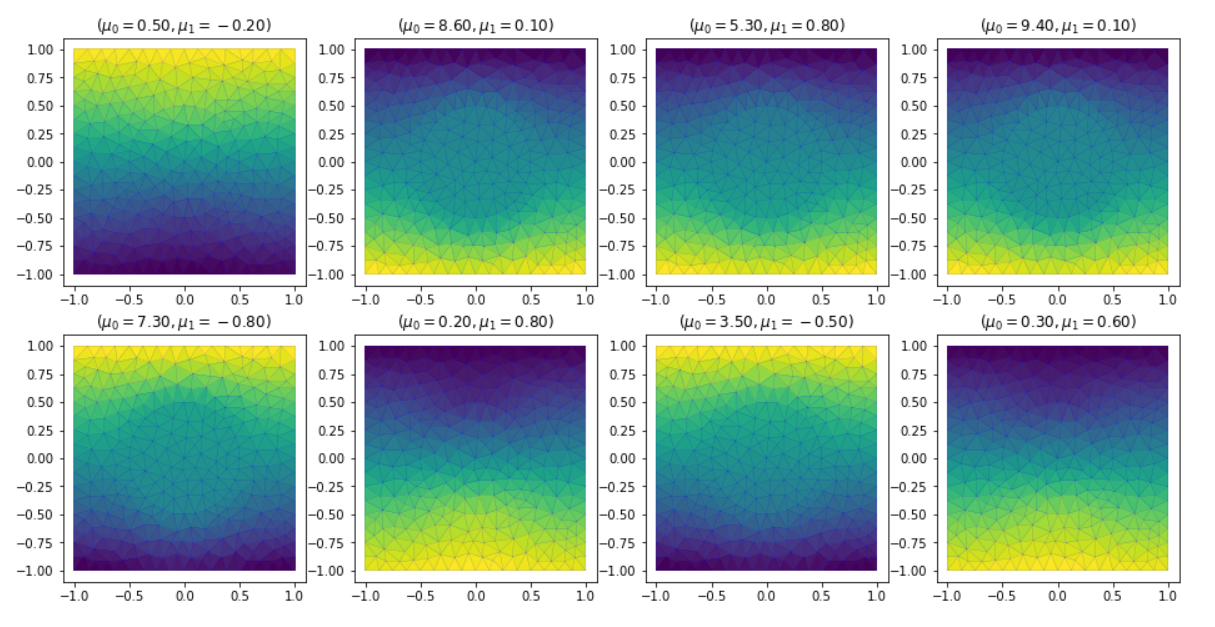
\includegraphics[width=\textwidth]{images/snapshots}
	\caption[Snapshots]{Heat distribution for the differen snapshots. }
	\label{fig:snaps}
\end{figure}

We created a reduced model from the snapshots using our algorithm.
In Figure \ref{fig:Singularvals} the value of the singular values respectively the square root of the eigenvalues is plotted.
We can see that the singular values shrink a lot between the first two modes. The following values are also shrinking but with a smaller magnitude than the first ones.

This behavior can be observed in practice. The first singular values have the biggest magnitude and decrease fast. The  modes with the singular values that fall no longer significantly can be truncated as discussed in Section \ref{sec:POD}. 

\begin{figure}[H]
	\centering
	% This file was created by matlab2tikz.
%
%The latest updates can be retrieved from
%  http://www.mathworks.com/matlabcentral/fileexchange/22022-matlab2tikz-matlab2tikz
%where you can also make suggestions and rate matlab2tikz.
%
\definecolor{mycolor1}{rgb}{0.00000,0.44700,0.74100}%
\definecolor{mycolor2}{rgb}{0.85000,0.32500,0.09800}%
\definecolor{mycolor3}{rgb}{0.92900,0.69400,0.12500}%
%
\begin{tikzpicture}

\begin{axis}[%
width=4.521in,
height=3.566in,
at={(0.758in,0.481in)},
scale only axis,
xmin=0.25,
xmax=8.25,
xlabel style={font=\color{white!15!black}},
xlabel={POD modes},
ymin=0,
ymax=950,
ylabel style={font=\color{white!15!black}},
ylabel={},
axis background/.style={fill=white},
axis x line*=bottom,
axis y line*=left,
legend style={at={(0.97,0.97)}, anchor=north east, legend cell align=left, align=left, draw=white!15!black}
]

\addplot [color=mycolor1, mark=+, mark options={solid, mycolor1, scale=2}]
table[row sep=crcr]{%
	1	874.5893 \\
	2	58.1832  \\
	3	48.2328  \\
	4	45.9105  \\
	5	35.5212  \\
	6	23.8663  \\
	7	20.6150  \\
	8	15.4926  \\
};
%\addlegendentry{Eigen values}

\end{axis}
\end{tikzpicture}%
	\caption[Singular values]{Singular values of the corresponding POD modes}
	\label{fig:Singularvals}
\end{figure}

For this simple example we didn't do the truncation.
Figure \ref{fig:reconstruct} shows a reconstucted solution with the parameter $ \bar{\mu} = (\bar{\mu}_1 , \bar{\mu}_2 )^T = ( 8 , 1 )^T $.
\begin{figure}[H]
	\centering
	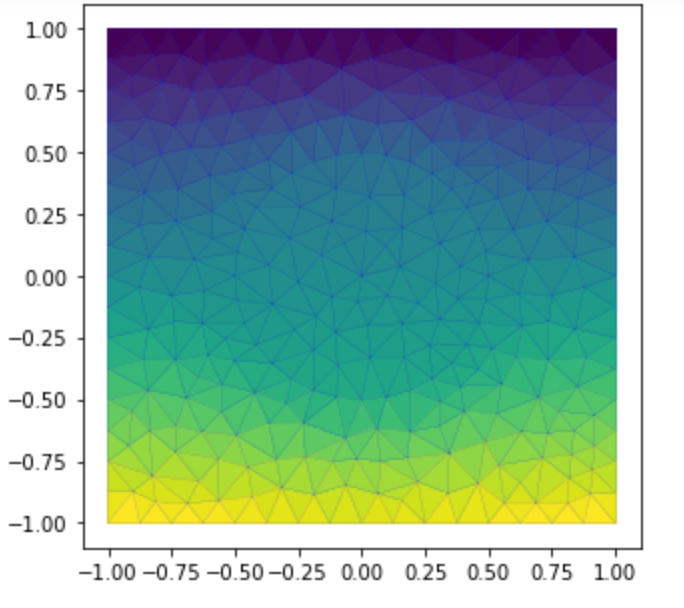
\includegraphics[width=0.38\textwidth]{images/reconstruct}
	\caption[Reduced Solution]{A solution computed with the reduced model created with \texttt{EZyRB}}
	\label{fig:reconstruct}
\end{figure}

\subsubsection{Benchmark}
With the data from tutorial 1 from \texttt{EZyRB} \cite{demo18ezyrb} we showed that the algorithm works properly, but it is not suitable to evaluate the performance.

To evaluate the performance we used a snapshot matrix with the same dimension as in Section \ref{sec:Benchmarks} and measured the time the POD class needs to compute the POD modes. This benchmark shows the performance we loose by using the python layer.

Due to issues with the cluster we had to do this benchmark on a different cluster. The new cluster has processors with 16 cores.
In Figure \ref{fig:ezybench} we can see that the measuring points increase in steps of 16 processors and not in steps of 10 like the benchmarks in Section \ref{sec:Benchmarks}.
We can still see that the implementation performed similar to the other benchmark in Figure \ref{fig:bench5} from Section \ref{sec:hybrid}.
\begin{figure}[H]
	\centering
	% This file was created by matlab2tikz.
%
%The latest updates can be retrieved from
%  http://www.mathworks.com/matlabcentral/fileexchange/22022-matlab2tikz-matlab2tikz
%where you can also make suggestions and rate matlab2tikz.
%
\definecolor{mycolor1}{rgb}{0.00000,0.44700,0.74100}%
\definecolor{mycolor2}{rgb}{0.85000,0.32500,0.09800}%
\definecolor{mycolor3}{rgb}{0.92900,0.69400,0.12500}%
%
\begin{tikzpicture}

\begin{axis}[%
width=4.521in,
height=3.566in,
at={(0.758in,0.481in)},
scale only axis,
xmin=0,
xmax=132,
xlabel style={font=\color{white!15!black}},
xlabel={Number of Processors},
ymin=0,
ymax=14.2,
ylabel style={font=\color{white!15!black}},
ylabel={Speed up},
axis background/.style={fill=white},
axis x line*=bottom,
axis y line*=left,
legend style={at={(0.03,0.97)}, anchor=north west, legend cell align=left, align=left, draw=white!15!black}
]

\addplot [color=mycolor3, mark=+, mark options={solid, mycolor3}]
table[row sep=crcr]{%
1     0.926193820542935\\
16    5.564527272810553\\
32    8.253695032798474\\
48    9.810377172379205\\
64    10.85966997160303\\
80    11.87933924922592\\
96    12.30403623120082\\
112   12.67579337348104\\
128   13.13623736917454\\
};
%\addlegendentry{EZyRB}




\end{axis}
\end{tikzpicture}%
	\caption[EZyRB Benchmark]{Benchmark integrated in the reduced order modeling framework \texttt{EZyRB}}
	\label{fig:ezybench}
\end{figure}


\newpage
\section{Conclusion}
We presented two algorithms to compute the POD in parallel.
A parallel algorithm using the singular value decomposition (SVD) and a parallel algorithm solving the eigenvalue problem of the correlation matrix (EVP).
Both algorithms performed good in case the snapshot matrix is already distributed to the different processors.
We saw that the EVP algorithm performs best, due to its limited number of operations.

For the case that the snapshot matrix is not distributed to the processors the algorithm got improved.
%We also tried to improve this algorithm for the case that the snapshot matrix is not yet distributed to the processors.
We proposed a hybrid implementation to overcome the number of communications.

Finally we  integrated the hybrid implementation into the reduced order modeling framework \texttt{EZyRB}.
We tested the new algorithm using \texttt{EZyRB} and also benchmarked the algorithm in the Python package.
With the parallel algorithm \texttt{EZyRB} can now make use af high perfomance cluster for the POD modes extraction.

In future works one could try to speed up the computation of the correlation matrix for the case that the snapshot matrix is not distributed.
Scattering the snapshot matrix to the processors is an expensive operation and slows down the overall POD computation a lot.
Instead of scattering the snapshot matrix to the processors, one could try to use Graphics Processing Units (GPU) for the computation of the correlation matrix.
GPUs are well suited these kine of operations.









\appendix
% hier Anhänge einbinden
\chapter{Appendix}
\section{POD module in C for Python}
\label{list:cPODpython}

The MPI wrapper is taken from \cite{DALCIN20051108}:\\
\href{https://bitbucket.org/mpi4py/mpi4py/src/73129d2c792291a735c47bca51684ae1d524a4aa/demo/wrap-c/?at=master}
{https://bitbucket.org/mpi4py/mpi4py/src/ \\73129d2c792291a735c47bca51684ae1d524a4aa/demo/wrap-c/?at=master}

We extended a numpy wrapper and included the POD algorithm.

\begin{lstlisting}

#define MPICH_SKIP_MPICXX 1
#define OMPI_SKIP_MPICXX  1
#include <Eigen/Dense>
#include <mpi4py/mpi4py.h>
#include "arrayobject.h"

using namespace Eigen;
typedef Matrix<double, -1, -1, RowMajor> Mat;
/* - Hybrid POD algorithem ------------------------------------------------- */

static void
master(MPI_Comm comm, PyArrayObject *wmatrix, PyArrayObject *umatrix) {
	
	if (comm == MPI_COMM_NULL) {
		printf("You passed MPI_COMM_NULL !!!\n");
		return;
	}
	// MPI: Who am i and how many
	int size; MPI_Comm_size(comm, &size);
	int rank; MPI_Comm_rank(comm, &rank);
	
	// Pointer to allocated Snapsotmatrix
	double * W = (double *)wmatrix->data;
	// Pinter to allocated POD vectors
	double * U = (double *)umatrix->data;
	
	// get dimention from numpy object
	int m,n;
	m = PyArray_DIM(wmatrix, 0);
	n = PyArray_DIM(wmatrix, 1);
	
	// allocate correlation matrix
	Mat CORR(n,n);
	
	// brodcast dimentions to all processors
	MPI_Bcast(&m, 1, MPI_INT, 0, comm);
	MPI_Bcast(&n, 1, MPI_INT, 0, comm);
	
	// calculate block sizes
	int nofrows = m / size;
	int remainder = m % size;
	if (rank < remainder) ++nofrows;
	
	int counts[size]; int displs[size];
	
	int offset = 0;
	for (int i = 0; i < size; ++i) {
		displs[i] = offset; 
		counts[i] = m / size;
		if (i < remainder) ++counts[i];
		
		counts[i] *= n; 
		offset += counts[i];
	}
	
	
	// initiate Self Adjoint Eigen Problem Solver
	Eigen::SelfAdjointEigenSolver<Mat> es;
	
	// allocate local matrices
	Mat w(nofrows, n);
	Mat sv(n,n);
	
	// Scatter snapshots
	MPI_Scatterv( W , counts , displs , MPI_DOUBLE ,
	w.data(), nofrows*n , MPI_DOUBLE ,
	0 , comm  );
	
	// compute local correaltion matrix
	Mat corr(n,n);
	corr.noalias() = w.transpose() * w; 
	
	// compute global correlation matrix
	MPI_Reduce(corr.data(), CORR.data(), n*n, MPI_DOUBLE,
	MPI_SUM, 0, comm);
	
	
	// solve eigenlvlaue problem
	es.compute(CORR);
	// work = V * S^-1
	sv = es.eigenvectors().rowwise().reverse().leftCols(n);
	for(int i=0; i<sv.cols(); i++){
		sv.col(i) *= 1.0/sqrt(es.eigenvalues().reverse().head(n)[i]);
	}
	
	// brodcast sv matrix
	MPI_Bcast(sv.data(), n*n, MPI_DOUBLE, 0, comm);
	
	// compute local pod vectors
	Mat u; 
	u.noalias() = w * sv; 
	
	// gather pod vectors
	MPI_Gatherv( u.data() , nofrows*n , MPI_DOUBLE , 
	U, counts ,  displs , MPI_DOUBLE ,
	0 , comm  );
	
	return;
}

static void
worker(MPI_Comm comm) {
	
	if (comm == MPI_COMM_NULL) {
		printf("You passed MPI_COMM_NULL !!!\n");
		return;
	}
	
	// MPI: Who am i and how many
	int size; MPI_Comm_size(comm, &size);
	int rank; MPI_Comm_rank(comm, &rank);
	
	// brodcast dimentions to all processors
	int m,n;	
	MPI_Bcast(&m, 1, MPI_INT, 0, comm);
	MPI_Bcast(&n, 1, MPI_INT, 0, comm);
	
	// calculate block sizes
	int nofrows = m / size;
	int remainder = m % size;
	if (rank < remainder) ++nofrows;
	
	int counts[size]; int displs[size];
	
	// allocate local matrices
	Mat w(nofrows, n);
	Mat sv(n,n);
	
	// recive local snapshots
	MPI_Scatterv( NULL , counts , displs , MPI_DOUBLE ,
	w.data(), nofrows*n , MPI_DOUBLE ,
	0 , comm  );
	
	// compute local correaltion matrix
	Mat corr(n,n);
	corr.noalias() = w.transpose() * w; 
	
	// compute global correlation matrix	
	MPI_Reduce(corr.data(), NULL, n*n, MPI_DOUBLE,
	MPI_SUM, 0, comm);
	
	// recive sv
	MPI_Bcast(sv.data(), n*n, MPI_DOUBLE, 0, comm);
	
	// compute local correlation matrix
	Mat u; 
	u.noalias() = w * sv; 
	
	//send local pod vecotrs
	MPI_Gatherv( u.data() , nofrows*n , MPI_DOUBLE , 
	NULL , counts ,  displs , MPI_DOUBLE ,
	0 , comm  );
	
	return;
}

/* - python wrapper functions-------------------------------------------- */

// Master Function called by python
static PyObject *
parapod_master(PyObject *self, PyObject *args)
{
	PyObject *py_comm;
	MPI_Comm *comm_p;
	PyArrayObject *wmatrix;
	PyArrayObject *umatrix;
	
	if (!PyArg_ParseTuple(args, "OOO:master", &py_comm, &wmatrix, &umatrix)) return NULL;
	
	comm_p = PyMPIComm_Get(py_comm);
	if (comm_p == NULL) return NULL;
	
	master(*comm_p, wmatrix, umatrix);
	
	Py_INCREF(Py_None);
	return Py_None;
}

// Worker Function called by python
static PyObject *
parapod_worker(PyObject *self, PyObject *args)
{
	PyObject *py_comm;
	MPI_Comm *comm_p;
	
	if (!PyArg_ParseTuple(args, "O:worker", &py_comm)) return NULL;
	
	comm_p = PyMPIComm_Get(py_comm);
	if (comm_p == NULL) return NULL;
	
	worker(*comm_p);
	
	Py_INCREF(Py_None);
	return Py_None;
}


static struct PyMethodDef parapod_methods[] = {
	{"master",   (PyCFunction)parapod_master,   METH_VARARGS, NULL},
	{"worker",   (PyCFunction)parapod_worker,   METH_VARARGS, NULL},
	{NULL,       NULL,                     0,            NULL} /* sentinel */
};

#if PY_MAJOR_VERSION < 3
/* --- Python 2 --- */

PyMODINIT_FUNC initparapod_module(void)
{
	PyObject *m = NULL;
	
	/* Initialize mpi4py C-API */
	//if (import_mpi4py() < 0) goto bad;
	if (import_mpi4py() < 0) return;
	
	/* Module initialization  */
	m = Py_InitModule("parapod", parapod_methods);
	if (m == NULL) goto bad;
	
	return;
	
	//bad:
	//return;
}

#else
/* --- Python 3 --- */

static struct PyModuleDef parapod_module = {
	PyModuleDef_HEAD_INIT,
	"parapod", /* m_name */
	NULL,         /* m_doc */
	-1,           /* m_size */
	parapod_methods    /* m_methods */,
	NULL,         /* m_reload */
	NULL,         /* m_traverse */
	NULL,         /* m_clear */
	NULL          /* m_free */
};

PyMODINIT_FUNC
PyInit_parapod(void)
{
	PyObject *m = NULL;
	
	/* Initialize mpi4py's C-API */
	if (import_mpi4py() < 0) return NULL;
	
	/* Module initialization  */
	m = PyModule_Create(&parapod_module);
	if (m == NULL) return NULL;
	
	return m;
}

#endif
\end{lstlisting}

\section{Waiting time BS 330}
\label{list:WTimeBS330}
\begin{lstlisting}
nodes=80 dofs=1000000 snapshots=300 bs=330
rank = 12  min = 0.0043131 max = 0.0249866
rank = 13  min = 0.0046517 max = 0.0242660
rank = 14  min = 0.0044078 max = 0.0240446
rank = 15  min = 0.0047344 max = 0.0241300
rank = 3   min = 0.0018230 max = 0.0247925
rank = 16  min = 0.0047779 max = 0.0245413
rank = 0   min = 0.0077286 max = 0.0135336
rank = 2   min = 0.0028240 max = 0.0250917
rank = 1   min = 0.0013872 max = 0.0214948
rank = 4   min = 0.0031843 max = 0.0247981
rank = 5   min = 0.0009631 max = 0.0252511
rank = 6   min = 0.0028348 max = 0.0271796
rank = 7   min = 0.0022160 max = 0.0245563
rank = 8   min = 0.0042824 max = 0.0255985
rank = 9   min = 0.0025902 max = 0.0258349
rank = 10  min = 0.0042816 max = 0.0229909
rank = 11  min = 0.0041316 max = 0.0235578
rank = 17  min = 0.0047368 max = 0.0243006
rank = 18  min = 0.0046265 max = 0.0246917
rank = 19  min = 0.0046437 max = 0.0271941
rank = 30  min = 0.0076763 max = 0.0314391
rank = 31  min = 0.0044388 max = 0.0293830
rank = 32  min = 0.0047194 max = 0.0298569
rank = 33  min = 0.0081659 max = 0.0307738
rank = 34  min = 0.0043481 max = 0.0297940
rank = 35  min = 0.0094767 max = 0.0307792
rank = 23  min = 0.0022570 max = 0.0297334
rank = 20  min = 0.0018981 max = 0.0291365
rank = 21  min = 0.0007308 max = 0.0275428
rank = 22  min = 0.0021548 max = 0.0276729
rank = 24  min = 0.0015231 max = 0.0311961
rank = 25  min = 0.0076888 max = 0.0296880
rank = 26  min = 0.0040453 max = 0.0311608
rank = 27  min = 0.0068116 max = 0.0312140
rank = 28  min = 0.0086282 max = 0.0316162
rank = 29  min = 0.0094516 max = 0.0294205
rank = 43  min = 0.0130634 max = 0.0232435
rank = 40  min = 0.0133841 max = 0.0241305
rank = 41  min = 0.0130425 max = 0.0254509
rank = 42  min = 0.0130218 max = 0.0256491
rank = 44  min = 0.0099885 max = 0.0290970
rank = 45  min = 0.0108420 max = 0.0290336
rank = 46  min = 0.0109732 max = 0.0285007
rank = 47  min = 0.0099189 max = 0.0284578
rank = 48  min = 0.0117451 max = 0.0279839
rank = 49  min = 0.0104234 max = 0.0286017
rank = 50  min = 0.0143602 max = 0.0229421
rank = 51  min = 0.0119498 max = 0.0275804
rank = 52  min = 0.0143473 max = 0.0228536
rank = 53  min = 0.0126253 max = 0.0269693
rank = 54  min = 0.0135484 max = 0.0262195
rank = 63  min = 0.0137158 max = 0.0233905
rank = 55  min = 0.0146116 max = 0.0235405
rank = 60  min = 0.0136492 max = 0.0233761
rank = 58  min = 0.0133206 max = 0.0265307
rank = 56  min = 0.0135418 max = 0.0278898
rank = 59  min = 0.0136631 max = 0.0282376
rank = 57  min = 0.0135731 max = 0.0291565
rank = 61  min = 0.0136313 max = 0.0282906
rank = 62  min = 0.0134978 max = 0.0237248
rank = 64  min = 0.0143792 max = 0.0231585
rank = 65  min = 0.0138563 max = 0.0283055
rank = 66  min = 0.0148908 max = 0.0268243
rank = 67  min = 0.0145527 max = 0.0234873
rank = 68  min = 0.0142011 max = 0.0237200
rank = 69  min = 0.0144420 max = 0.0284821
rank = 70  min = 0.0144735 max = 0.0238491
rank = 71  min = 0.0141707 max = 0.0241045
rank = 72  min = 0.0143723 max = 0.0287977
rank = 73  min = 0.0142900 max = 0.0239163
rank = 74  min = 0.0145044 max = 0.0242005
rank = 75  min = 0.0143538 max = 0.0241516
rank = 79  min = 0.0136074 max = 0.0283309
rank = 76  min = 0.0133768 max = 0.0282639
rank = 77  min = 0.0136647 max = 0.0295025
rank = 78  min = 0.0135516 max = 0.0255812
rank = 36  min = 0.0127170 max = 0.0241173
rank = 37  min = 0.0110443 max = 0.0255328
rank = 38  min = 0.0128222 max = 0.0243029
rank = 39  min = 0.0128500 max = 0.0239090
\end{lstlisting}

\backmatter
\printbibliography

\clearpage
\thispagestyle{empty}

Name: \fullname \hfill Matrikelnummer: \matnr \vspace{2cm}
%Name: \fullname \hfill matriculation number : \matnr \vspace{2cm}

%\minisec{Erklärung}
%Ich erkläre, dass ich die Arbeit selbständig verfasst und keine anderen als die angegebenen Quellen und Hilfsmittel verwendet habe.\vspace{2cm}
\minisec{Declaration}

I declare that I have written the work independently and have not used any other sources and aids than those cited.\vspace{1.5cm}
\begin{figure}[H]
\hspace{8.75cm}

\includegraphics[width=0.3\textwidth]{images/Fueller2.1.png}
\end{figure}
\vspace{-1.3cm}
Ulm, \today, \dotfill

\hspace{10cm} {\footnotesize \fullname}
\end{document}
